% 150 câu đã gỡ khỏi ngân hàng (chuyen_dang) — chép lại vào file dạng để khôi phục

% từ: cau-hoi/lop10/0D1_Menh_de_Tap_hop/0D1-3-4_Hieu_va_phan_bu_dung_doan_khoang.tex
\begin{ex}%[0D1Y3-4]%[ma:3113212d]
	Một cửa hàng bán áo sơ mi thống kê  số lượng áo bán ra trong tháng $ 1 $ như bảng sau.
	\begin{center}
		\begin{tabular}{|c|l|l|l|l|l|l|}
			\hline Cơ áo & 37 & 38 & 39 & 40 & 41 &  42 \\
			\hline Số lượng & 35 & 42 & 50  & 38 & 32 & 48 \\
			\hline 
		\end{tabular}
	\end{center}
	Mốt của mẫu số liệu trên  bằng?
	\choice 
		 {$ 42 $}
		{$ 39 $} 
		 {$ 41 $}
		{\True $  50 $}
	 \loigiai{
		Mốt của mẫu số  liệu trên là $ 50 $.
	 }
\end{ex}

% từ: cau-hoi/lop10/0D3_Ham_so_bac_hai_va_do_thi/0D3-1-1_Xac_dinh_mot_ham_so.tex
\begin{ex}%[0D3Y1-1]%[ma:caa9b60e]
	Gieo một đồng xu cân đối và đồng chất 2 lần. Số phần tử của không gian mẫu là 
	\choice 
		{$  8 $}
		{$  6 $}
		{\True  $ 4 $}
		{$ 2 $ } 
	 \loigiai{
		Số  phần tử không gian mẫu $ n\left(\Omega\right) =4$.
	 }
\end{ex}

% từ: cau-hoi/lop10/0D3_Ham_so_bac_hai_va_do_thi/0D3-1-2_Tap_xac_dinh_cua_ham_so.tex
\begin{ex}%[0D3N1-2]%[ma:e5208705]
	Cặp số nào sau đây là nghiệm của hệ  bất phương trình $\heva{& x+2y\le8\\ & 3x-y>3 }$ ?
	\choice 
		 {$\left(0; 4\right)$ }
		 {$\left(1; 1\right)$}
		 {\True $\left(4; 1\right)$}
		{$\left(2;  3\right)$}
	 \loigiai{
		Lần lượt thay các  bộ số vào hệ bất phương trình ta được một nghiệm của hệ bất phương trình trên là $\left(4; 1\right)$.
	} 
\end{ex}

% từ: cau-hoi/lop10/0D3_Ham_so_bac_hai_va_do_thi/0D3-1-2_Tap_xac_dinh_cua_ham_so.tex
\begin{ex}%[0D3N1-2]%[ma:b32aac76]
	Cho hệ bất phương  trình $\heva{& 2x-5y-1>0 \\& 2x+y+5>0\\&x+y+1<0}$. Trong các điểm sau, điểm nào thuộc miền nghiệm của hệ bất phương trình?
	\choice 
		 {$O\left(0;0\right)$}
		 {$M\left(1;0\right)$}
		{\True  $N\left(0;-2\right)$}
		 {$P\left(0;2\right)$}
	 \loigiai{
		Ta thay lần lượt tọa độ các điểm vào hệ bất phương  trình.\\
		Ta thấy điểm $N\left(0;-2\right)$ thỏa mãn hệ. 
	} 
\end{ex}

% từ: cau-hoi/lop10/0D3_Ham_so_bac_hai_va_do_thi/0D3-1-2_Tap_xac_dinh_cua_ham_so.tex
\begin{ex}%[0D3N1-2]%[ma:27f88824]
	Cho hệ bất phương trình $\heva{& x+3y-2\ge0\\ & 2x+y+1\le0 }$. Trong các điểm sau, điểm nào  thuộc miền nghiệm của hệ bất phương trình?
	\choice 
		{$M\left(0;1\right)$} 
		{\True  $N\left(-1;1\right)$}
		 {$P\left(1;3\right)$}
		{$Q\left(2;1\right)$} 
	\loigiai{ 
		Ta thay lần lượt tọa độ các điểm vào hệ  bất phương trình.\\
		Ta thấy $N\left(-1;1\right)$ thỏa  mãn.
	 }
\end{ex}

% từ: cau-hoi/lop10/0D3_Ham_so_bac_hai_va_do_thi/0D3-1-2_Tap_xac_dinh_cua_ham_so.tex
\begin{ex}%[0D3N1-2]%[ma:a3ab6552]
	Miền nghiệm của hệ bất phương trình  $\heva{& x>0 \\& x-y\le2\\&x+y\le1}$ chứa điểm nào sau đây?
	\choice 
		{\True $A\left(\dfrac{1}{2};-1\right)$} 
		 {$B\left(1;2\right)$}
		 {$C\left(0;2\right)$}
		 {$D\left(3;-2\right)$}
	 \loigiai{
		Thay tọa độ điểm $A\left(\dfrac{1}{2};-1\right)$  vào hệ phương trình ta thấy thỏa mãn.\\
		Suy ra điểm $A\left(\dfrac{1}{2};-1\right)$ thuộc miền nghiệm của hệ bất phương trình đã cho. 
	 }
\end{ex}

% từ: cau-hoi/lop10/0D3_Ham_so_bac_hai_va_do_thi/0D3-1-2_Tap_xac_dinh_cua_ham_so.tex
\begin{ex}%[0D3Y1-2]%[ma:461f34c2]
	Gieo một con xúc xắc cân đối và đồng chất ba lần. Số  phần tử của không gian mẫu là
	 \choice
		 {\True $6^3$}
		 {$6^2$}
		{$6$} 
		 {$6^4$}
	 \loigiai{
		Ta có $n\left(\Omega\right)=6\cdot 6\cdot 6=6^3$. 
	 }
\end{ex}

% từ: cau-hoi/lop10/0D3_Ham_so_bac_hai_va_do_thi/0D3-1-5_Tinh_dong_bien_nghich_bien.tex
\begin{ex}%[0D3H1-5]%[ma:bb1a2cfa]
	Cho hệ bất phương trình $\heva{&  x+ y -2\leq 0 \\& 2 x-3 y +2>0}$.
	\choiceTF 
		{\True Hệ trên  là một hệ bất phương trình bậc nhất hai ẩn}
		{$\left(-1; 3\right)$ là một nghiệm của hệ bất phương trình trên} 
		 {\True $\left(1; 1\right)$ là một nghiệm của hệ bất phương trình trên}
		 {$\left(2; -2\right)$ không là một nghiệm của hệ bất phương trình trên}
	\loigiai{ 
		\begin{itemchoice}
			\itemch Hệ trên là một hệ bất  phương trình bậc nhất hai ẩn.
			\itemch Thay $x=-1; y=3$ vào hệ bất phương trình ta được $\heva{&0\ge0\\&-9>0}$ (Vô lý).\\ Vậy $\left(-1; 3\right)$ không phải là một nghiệm của  hệ bất phương trình.
			\itemch Thay $x=1; y=1$  vào hệ bất phương trình ta được $\heva{&0\le0\\&1>0}$ (luôn đúng).\\ Vậy $\left(1; 1\right)$ là một nghiệm của hệ bất phương trình.
			\itemch Thay $x=2; y=-2$ vào hệ bất phương trình ta được $\heva{&-2\le0\\&12>0}$ (luôn đúng).\\ Vậy $\left(2; -2\right)$ là một  nghiệm của hệ bất phương trình.
		\end{itemchoice}
	} 
\end{ex}

% từ: cau-hoi/lop10/0D3_Ham_so_bac_hai_va_do_thi/0D3-1-5_Tinh_dong_bien_nghich_bien.tex
\begin{ex}%[0D3H1-5]%[ma:c5c38282]
	Cho hệ bất phương  trình $\heva{&x+2y-100 \leq 0\\&2x+y-80\leq0\\&x\geq 0\\&y\geq 0}$.
	\choiceTF 
		{Hệ trên không phải là một hệ bất phương trình bậc nhất hai ẩn} 
		{$\left(-1; 2\right)$ là một nghiệm của hệ bất phương  trình trên}
		{\True $\left(-1; 5\right)$ không  là một nghiệm của hệ bất phương trình trên}
		{\True Miền nghiệm của  hệ bất phương trình trên là một miền tứ giác}
	 \loigiai{
		\begin{itemchoice}
			\itemch Vì hệ trên là  một hệ bất phương trình bậc nhất hai ẩn.
			\itemch Vì thay $x=-1; y=2$ vào hệ bất phương trình ta được $\heva{-97 &\leq 0\\-80&\leq0\\-1&\geq 0\\2&\geq 0} $ (Vô lý).\\ Vậy $\left(-1; 2\right)$ không phải là một nghiệm của  hệ bất phương trình.
			\itemch Thay $x=-1; y=5$ vào hệ bất phương trình ta được $\heva{&-91 \leq 0\\&-77\leq0\\&-1\geq 0\\&5\geq  0} $ (Vô lý).\\ Vậy $\left(-1; 5\right)$ không là một nghiệm của hệ bất phương trình.
			\itemch Vẽ  đường thẳng $d_1:x+2y-100=0$. Vì $0+2\cdot0-100\leq0$ nên toạ độ điểm $O\left(0; 0\right)$ thoả mãn bất phương trình $:x+2y-100\leq0$. Do đó miền nghiệm $D_1$ của bất phương trình $x+2y-100\leq0$ là nửa mặt phẳng bờ $d_1:x+2y-100=0$ chứa gốc toạ độ $O$.\\
			Tương tự miền nghiệm $D_2$ của bất phương trình $2x+y-80\leq0$ là nửa mặt phẳng bờ $d_2:2x+y-80=0$ chứa gốc toạ độ $O$.\\ 
			Tương tự miền nghiệm $D_4$ của bất  phương trình $x\geq0$ là nửa mặt phẳng bờ $Oy$ chứa điểm $\left(1; 0\right)$.\\
			Tương tự miền nghiệm $D_3$ của bất phương trình $y\geq0$ là nửa  mặt phẳng bờ $Ox$ chứa điểm $\left(0; 1\right)$.\\
			Khi đó miền nghiệm của  hệ bất phương trình là miền tứ giác $OABC$.
			\begin{center}
				\begin{tikzpicture}[scale=0.6,thick,>=stealth']
						\draw[->]  (-3,0) -- (12,0) node[above]{$x$};
						 \draw[->,color=black] (0,-2) -- (0,9) node[right]{$y$};
						\node[below left] at  (0,0) {$O$};
						\clip  (-3,-2) rectangle (12,9);
						\draw[line width=1.2pt,smooth,samples=100,domain=-1:9] plot  (\x,{-2*(\x)+8});
						\draw[line width=1.2pt,smooth,samples=100,domain=-1:15.3] plot (\x,{-0.5*(\x)+5}); 
						\fill[pattern=north east lines] (0,0)--(0,5)  --(2,4)--(4,0)-- cycle;
						\node[above]  at (4,0) {$A$};
						 \node[below] at (4,0) {$40$}; \node[below] at (10,0) {$100$};
						\node[right] at (0,5)  {$B$}; \node[left] at (0,5) {$50$};
						\node[left] at (0,8)  {$80$};
						\node[right] at (2,4)  {$C$}; \node[left] at (0,4) {$40$};
						\node[below] at (2,0) {$20$};  \draw[dashed] (0,4)--(2,4)--(2,0);
					\end{tikzpicture}
			\end{center}
		\end{itemchoice}
	} 
\end{ex}

% từ: cau-hoi/lop10/0D3_Ham_so_bac_hai_va_do_thi/0D3-2-1_Xac_dinh_ham_so_bac_hai.tex
\begin{ex}%[0D3N2-1]%[ma:05982543]
	Trong các biểu  thức sau, biểu thức nào là tam thức bậc 2?
	 \choice
		{\True $f_1(x)  = 15x^2 - 10$}
		{$f_2(x) = \sqrt{6x^2 + 15x  - 10}$}
		{$f_3(x)  = 15x - 10 + \dfrac{1}{x^2}$}
		{$f_4(x)  = 6x + 9$}
	 \loigiai{
		Tam thức  bậc hai có dạng tổng quát là $ ax^2 + bx + c $ với $ a \neq 0 $.\\
		Vậy đáp án  đúng là $ f_1(x) = 15x^2 - 10 $.
	 }
\end{ex}

% từ: cau-hoi/lop10/0D3_Ham_so_bac_hai_va_do_thi/0D3-2-1_Xac_dinh_ham_so_bac_hai.tex
\begin{ex}%[0D3H2-1]%[ma:2c950d59]
	 Hàm số $y=-x^2+2x-5$ đồng biến trên khoảng
	\choice 
		 {$(-\infty;-1)$}
		 {$(-1;+\infty)$}
		{\True $(-\infty;1)$} 
		{$(1;+\infty)$} 
	\loigiai{ 
		Vì hàm số $y=-x^2+2x-5$ là hàm số bậc hai có $a=-1 < 0$ và hoành độ đỉnh $-\dfrac{b}{2a}=1$  nên hàm số đồng biến trên $(-\infty;1)$.
	} 
\end{ex}

% từ: cau-hoi/lop10/0D3_Ham_so_bac_hai_va_do_thi/0D3-2-2_Bang_bien_thien_tinh_don_dieu_max_min.tex
\begin{ex}%[0D3N2-2]%[ma:46aa1020]
	Hàm số $y=x^2-8x+12$ nghịch  biến trên khoảng
	\choice 
		{$(8;+\infty)$} 
		{$(-\infty;8)$} 
		{\True  $(-\infty;4)$}
		{$(4;+\infty)$} 
	 \loigiai{
		 Hàm số $y=x^2-8x+12$ có hệ số $a=1>0$ nên hàm số nghịch biến trên khoảng $\left(-\infty;-\dfrac{b}{2a}\right)$.\\
	Vì vậy hàm số  đã cho nghịch biến trên $(-\infty;4)$.}
\end{ex}

% từ: cau-hoi/lop10/0D3_Ham_so_bac_hai_va_do_thi/0D3-2-2_Bang_bien_thien_tinh_don_dieu_max_min.tex
\begin{ex}%[0D3H2-2]%[ma:d7a51d66]
	Hàm số $y=x^2-4x+11$ đồng biến  trên khoảng nào trong các khoảng sau đây?
	 \choice
		 {$(-2;+\infty)$}
		{$(-\infty;+\infty)$} 
		 {\True$(2;+\infty)$}
		{$(-\infty;2)$} 
	\loigiai{ 
		Ta có  bảng biến thiên
		\begin{center}
			
\begin{tikzpicture}
					\tkzTabInit[nocadre=true,lgt=1,espcl=2.5,deltacl=0.5] 
						 {$x$/0.7,$y$/2}
						 {$-\infty$,$2$,$+\infty$}
					 \tkzTabVar{+/$+\infty$,-/$7$,+/$+\infty$}
				\end{tikzpicture}
		\end{center}
		Từ  bảng biến thiên ta thấy, hàm số đồng biến trên khoảng $(2;+\infty)$.
	} 
\end{ex}

% từ: cau-hoi/lop10/0D7_Bat_phuong_trinh_bac_2_mot_an/0D7-2-1_Bat_phuong_trinh_bac_2_va_ung_dung.tex
\begin{ex}%[0D7H2-1]%[ma:c57303c8]
	\immini 
	{Cho hàm số bậc hai $f(x)=ax^2+bx+c$ với $a\ne  0$ có đồ thị như hình vẽ bên.
	 \choiceTF
		{Hàm số  đồng biến trên khoảng $(-2;-1)$}
		{Giá trị nhỏ nhất của  hàm số là $-1$}
		{\True $2a+b+c=3$.} 
		{\True $f(x)\leq  2$ với mọi $x\in [-3;1]$}}
		{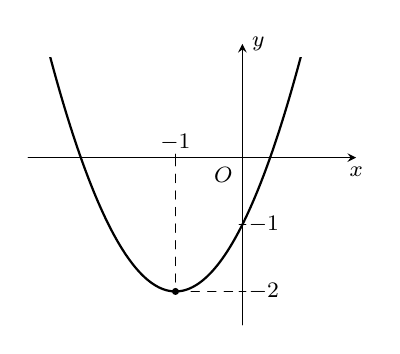
\begin{tikzpicture}[scale=0.85,line join=round,line cap=round,>=stealth,font=\footnotesize]
		\def\xmin{-3}\def\xmax{1.5}\def\ymin{-2.3}\def\ymax{1.5} 
		\draw[->] (\xmin-0.2,0)--(\xmax+0.2,0) node[below]{$x$}; 
		\draw[->] (0,\ymin-0.2)--(0,\ymax+0.2) node[right]{$y$}; 
		\draw (0,0) node[below left]{$O$}; 
		\draw (-1,0.05)--(-1,-0.05) node[above]{$-1$}; 
		\foreach \y  in {-2,-1}\draw (0.05,\y)--(-0.05,\y) node[right]{$\y$};
		\clip  (\xmin,\ymin) rectangle (\xmax,\ymax);
		\draw[thick,smooth,samples=200,domain=\xmin:\xmax]  plot (\x,{(\x)^2+2*(\x)-1});
		 \draw[dashed] (-1,0)--(-1,-2)--(0,-2); \fill (-1,-2) circle (1.5pt);
	\end{tikzpicture}
		 }
	 \loigiai{
		\begin{itemchoice}
			 \itemch Hàm số đồng biến trên khoảng $(-1;+\infty)$.
			\itemch Hàm số đạt giá trị nhỏ nhất bằng  $-2$ tại $x=-1$.
			\itemch Đồ thị hàm số đi qua $(0;-1)$ và có tọa độ đỉnh $(-1;-2)$  nên
			$$\heva{&c=-1\\& -\dfrac{b}{2a}=-1\\& a-b+c=-2} \Leftrightarrow \heva{&c=-1\\&2a-b=0\\&a-b+c=-2}  \Leftrightarrow \heva{&a=1\\&b=2\\&c=-1} \Rightarrow 2a+b+c=3 \Rightarrow f(x)=x^2+2x-1.$$
			\itemch Ta có $f(x)\leq 2 \Leftrightarrow  x^2+2x-1\leq 2 \Leftrightarrow x^2+2x-3\leq 0 \Leftrightarrow -3\leq x\leq 1$.
	\end{itemchoice}}
\end{ex}

% từ: cau-hoi/lop10/0D7_Bat_phuong_trinh_bac_2_mot_an/0D7-3-6_Toan_hinh_toan_thuc_te_ung_dung_phuong_trinh.tex
\begin{bt}%[0D7V3-6]%[ma:511a5c1b]
	Cho tam giác $ABC$ vuông tại  $A$, cạnh $AB$ ngắn hơn cạnh $AC$ là $2$. Biết chu vi của tam giác $ABC$ bằng $24$. Tính diện tích của tam giác $ABC$.\shortans{24}
	 \loigiai{
		Đặt $AB=x$, vì  cạnh $AB$ ngắn hơn cạnh $AC$ là $2$ nên độ dài cạnh $AC=AB+x=2+x$.\\
		Chu vi của tam  giác $ABC$ bằng $24$ nên
	\immini{			\begin{eqnarray*}
		 & & AB+BC+CA=24\\
		&\Leftrightarrow & x+\sqrt{2x^2+4x+4}+2+x=24  \\
		&\Leftrightarrow& \sqrt{2x^2+4x+4}=22-2x \qquad \qquad  \qquad (*)\\
		&\Rightarrow  & 2x^2+4x+4=484-88x+4x^2\\
		&\Rightarrow&  2x^2-92x+480=0\\
		&\Rightarrow  & x=40\ \text{hoặc}\ x=6.
	\end{eqnarray*}}
	{\begin{tikzpicture}[line join = round,line cap = round,>=stealth,font=\footnotesize,scale=0.9]
		\coordinate [label=left:$A$]  (A) at (0,0);
		\coordinate [label=above:$B$](B) at  (0,2);
		 \coordinate [label=below:$C$] (C) at (4,0);
		\draw (A)--(B)--(C)--(A); 
		\draw pic[draw,angle radius=2mm]  {right angle = B--A--C};
		\foreach  \diem in {A,B,C} \fill (\diem) circle (1.5pt);
	\end{tikzpicture}
	 }
	Thay lần lượt $x=40$, $x=6$ vào phương trình $(*)$, ta thấy chỉ có  $x=6$ thỏa mãn. \\
	Do đó phương trình  $(*)$ có nghiệm $x=6$.\\
	Khi đó độ dài ba cạnh của tam  giác $ABC$ là $AB=6$, $AC=8$, $BC=10$.
	\\ 
	Vậy diện tích tam giác $ABC$ là $S_{\triangle ABC}=\dfrac{1}{2}\cdot AB\cdot AC =  24$ (đ.v.d.t).
} 
\end{bt}

% từ: cau-hoi/lop10/0H9_Phuong_phap_toa_do_trong_mat_phang/0H9-1-3_Toa_do_diem_va_vecto_tren_he_truc_Oxy.tex
\begin{bt}%[0H9H1-3]%[ma:fc07e4aa]
	Cho hình thang cân $ABCD$ với $A(2; 0)$, $B(0;  2)$, $C(0; 7)$, $D(a;b)$. Tìm giá trị nhỏ nhất của $a+b$.
	 \loigiai{
		Gọi $D(x;  y)$ suy ra $\overrightarrow{CD}=(x;y-7)$, $\overrightarrow{AD}=(x-2;y)$.\\
		$\overrightarrow{AB}=(-2;2)\Rightarrow  AB=2\sqrt{2}$, $\overrightarrow{BC}=(0;5)\Rightarrow BC=5$.
		\begin{center}
			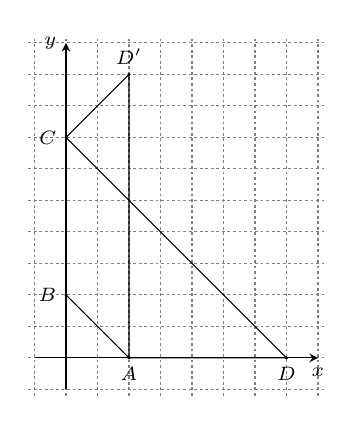
\begin{tikzpicture}[>=stealth,x=1cm,y=1cm,scale=0.4]
					 \def\a{-2}
					 \def\b{3}
					\draw[color=gray,dash pattern=on 1pt  off 1pt,xstep=1.0cm,ystep=1.0cm] (-1.2,-1.2) grid (8.2,10.2);
					\draw[->] (-1,0) -- (8,0) node[below] {\scriptsize  $x$};
					\draw[->] (0,-1) -- (0,10)  node[left] {\scriptsize $y$};
					\coordinate[label=below:\scriptsize $A$] (A) at (2,0); 
					\coordinate[label=left:\scriptsize $B$] (B)  at (0,2);
					\coordinate[label=left:\scriptsize $C$] (C) at  (0,7);
					\coordinate[label=below:\scriptsize $D$] (D) at (7,0); 
					 \coordinate[label=above:\scriptsize $D'$] (D') at (2,9);
					\draw (A)--(B)--(C)--(D)--(A) 
						 (A)--(B)--(C)--(D')--(A);
					\foreach \diem in {A,B,C,D,D'}\fill (\diem)  circle (1.5pt);
				\end{tikzpicture}
		\end{center}
		Trường hợp 1: Hình thang có hai  đáy $A B$, $C D$.\\
		Ta có $\heva{&\overrightarrow{AB},\overrightarrow{CD}\text{  cùng phương}\\&AD=BC}\Leftrightarrow\heva{&\dfrac{x}{-2}=\dfrac{y-7}{2} \\&\sqrt{(x-2)^2+y^2}=5} \Leftrightarrow\heva{&x=-y+7 \\&(-y+7-2)^2+y^2=25}$\\
		$\Leftrightarrow\heva{&x=-y+7 \\&2 y^2-10 y+25=25} \Leftrightarrow\heva{&x=7 \\&y=0} \ \text{hoặc}\ \heva{&x=2 \\&y=5.}$\\ 
		Với $\heva{&x=7 \\&y=0}$ thì  $CD=\sqrt{7^2+(0-7)^2}=7 \sqrt{2} \neq AB$ nên $D(7; 0)$ thỏa mãn.\\
		Với $\heva{&x=2 \\&y=5}$ thì $CD=\sqrt{2^2+(5-7)^2}=2 \sqrt{2}=AB$  (loại).\\
		Trường  hợp 2: Hình thang có hai đáy $BC$, $AD$.\\
		Ta có  $\heva{&\overrightarrow{BC},\overrightarrow{AD}\text{ cùng phương}\\&AB=CD}\Leftrightarrow\heva{&\dfrac{0}{x-2}=\dfrac{5}{y} \\&2\sqrt{2}=\sqrt{x^2+(y-7)^2}} \Leftrightarrow\heva{&\dfrac{x-2}{y}=\dfrac{0}{5} \\&x^2+(y-7)^2=8}$\\
		$\Leftrightarrow\heva{&x=2 \\&(y-7)^2=4} \Leftrightarrow\heva{&x=2 \\&y=5} \ \text{hoặc}\  \heva{&x=2 \\&y=9.}$\\
		 Với $\heva{&x=2 \\&y=9}$ thì $AD=\sqrt{0^2+9^2}=9 \neq BC$ nên $D(2;9)$ thỏa mãn.\\
		Với $\heva{&x=2  \\&y=5}$ thì $AD=\sqrt{0^2+5^2}=5=BC$ (loại).\\
		Vậy giá trị nhỏ nhất của  $a+b$ là $7$.
	 }
\end{bt}

% từ: cau-hoi/lop10/0H9_Phuong_phap_toa_do_trong_mat_phang/0H9-4-1_Tim_tam_ban_kinh_va_dieu_kien_la_duong_tron.tex
\begin{bt}%[0H9B4-1]%[ma:65caa0f3]
	Trong mặt phẳng tọa độ $Oxy$, lập phương trình chính tắc của Elip có độ dài trục lớn  là $8$, tiêu cự bằng $2\sqrt{5}$.
	\loigiai{ 
		Theo giả thiết, ta có $\heva{&2a = 8 \Rightarrow a = 4\\&2c = 2\sqrt{5}\Rightarrow c =  \sqrt{5}.}$\\
		Khi đó $b=\sqrt{a^2 - c^2}=\sqrt{16 - 5}=\sqrt{11}$.\\ 
		 Vậy phương trình Elip cần tìm là
		\[\dfrac{x^2}{a^2} + \dfrac{y^2}{b^2} = 1 \Leftrightarrow \dfrac{x^2}{16}+ \dfrac{y^2}{11}=1.\] 
	 }
\end{bt}

% từ: cau-hoi/lop10/0H9_Phuong_phap_toa_do_trong_mat_phang/0H9-4-2_Phuong_trinh_duong_tron.tex
\begin{bt}%[0H9Y4-2]%[ma:4ea01bed]
	Trong mặt phẳng tọa độ  $Oxy$, viết phương trình chính tắc của elip $(E)$ biết tiêu cự bằng $18$ và độ dài trục lớn bằng $24$.
	 \loigiai{
		Giả sử $(E)\colon \dfrac{x^2}{a^2}+\dfrac{y^2}{b^2} = 1$ là phương trình  elip cần tìm.\\
		Vì $(E)$ có tiêu cự bằng $18$ nên $2c=18$ suy ra $c=9$.\\ 
		Vì $(E)$ có độ dài trục lớn bằng $24$ nên $24=2a$ suy ra  $a=12$.\\
		Ta cũng  có $b=\sqrt{a^2-c^2}=3\sqrt{7}$.\\
		Vậy  $(E) \colon \dfrac{x^2}{144}+\dfrac{y^2}{63}=1$.
	} 
\end{bt}

% từ: cau-hoi/lop11/1D1_Ham_so_luong_giac_va_phuong_trinh_luong/1D1-1-1_Cau_hoi_ly_thuyet.tex
\begin{ex}%[1D1H1-1]%[ma:c27494b3]
 Cho  $\cos\alpha=\dfrac{2}{3}$ và $0<\alpha<\dfrac{\pi}{2}$.
 \choiceTF 
   {$\sin\alpha<0$}
  {\True  $\tan\alpha>0$}
  {\True  $\cot(\pi-\alpha)<0$}
   {\True $\sin2\alpha>0$}
  \loigiai{
  \begin{enumerate}
   \item  \textbf{Sai.}
   Do $0<\alpha<\dfrac{\pi}{2}$ là góc phần tư thứ nhất, nên $\sin\alpha>0$. 
    \item \textbf{Đúng.}
   Do $0<\alpha<\dfrac{\pi}{2}$ là góc phần tư thứ  nhất, nên $\tan\alpha>0$.
   \item \textbf{Đúng.} 
   Do $0<\alpha<\dfrac{\pi}{2}$ là góc phần  tư thứ nhất, nên $\cot\alpha>0$.\\ Mặt khác, $\cot(\pi-\alpha)=-\cot\alpha$ nên $\cot(\pi-\alpha)<0$.
   \item  \textbf{Đúng.}
   Do $0<\alpha<\dfrac{\pi}{2}$ là góc phần  tư thứ nhất, nên $\sin\alpha>0$ và $\cos\alpha>0$. Mặt khác, $\sin2\alpha=2\sin\alpha\cos\alpha$ nên $\sin2\alpha>0$.\\[-3mm]
  \end{enumerate}
  }
\end{ex}

% từ: cau-hoi/lop11/1D1_Ham_so_luong_giac_va_phuong_trinh_luong/1D1-1-2_Chuyen_doi_don_vi_do_va_radian.tex
\begin{ex}%[1D1N1-2]%[ma:b6e18f34]
	Giả sử các đẳng  thức đều có nghĩa. Chọn khẳng định đúng trong các khẳng định sau.
	 \choice
		{$\sin^2  \alpha+\cos^2\alpha=-1$}
		{\True $\tan \alpha \cdot  \cot \alpha=1$}
		{$1+\tan^2 \alpha=\dfrac{1}{\sin^2\alpha}$} 
		 {$1+\cot^2 \alpha=\dfrac{1}{\cos^2\alpha}$}
	 \loigiai{Theo tính chất ta có
		\begin{enumerate}
			 \item $\sin^2 \alpha+\cos^2\alpha=1$.
			\item $\tan \alpha \cdot \cot \alpha=1$. 
			\item $1+\tan^2  \alpha=\dfrac{1}{\cos^2\alpha}$.
			 \item $1+\cot^2 \alpha=\dfrac{1}{\sin^2\alpha}$.
		\end{enumerate}
	} 
\end{ex}

% từ: cau-hoi/lop11/1D1_Ham_so_luong_giac_va_phuong_trinh_luong/1D1-1-3_So_do_cua_mot_goc_luong_giac.tex
\begin{ex}%[1D1N1-3]%[ma:214989ec]
	Tìm  khẳng định \textbf{sai} trong các khẳng định sau đây?
	\choice 
		{$\tan  45{^\circ}<\tan 60{^\circ}$}
		{$\cos 45^\circ \le \sin  45{^\circ}$}
		{$\sin  60{^\circ}<\sin 80{^\circ}$}
		 {\True $\cos 35^\circ >\cos 10^\circ $}
	\loigiai{ 
	Khi $\alpha \in (0{^\circ};90{^\circ})$ hàm $\cos \alpha $ là hàm giảm nên $\cos 35^\circ <\cos 10^\circ $.  Suy ra $\cos 35^\circ >\cos 10^\circ $ sai.}
\end{ex}

% từ: cau-hoi/lop11/1D1_Ham_so_luong_giac_va_phuong_trinh_luong/1D1-1-4_Do_dai_cua_mot_cung_tron.tex
\begin{ex}%[1D1N1-4]%[ma:c7e4d922]
	Cho $2\pi <\alpha <\dfrac{5\pi}{2}$.  Chọn mệnh đề đúng.
	\choice 
		 {\True $\tan \alpha >0$}
		{$\cot  \alpha <0$}
		{$\sin \alpha  <0$}
		 {$\cos \alpha <0$}
	\loigiai{ 
	Ta có  $2\pi <\alpha <\dfrac{5\pi}{2}$ nên $\tan \alpha >0$.}
\end{ex}

% từ: cau-hoi/lop11/1D1_Ham_so_luong_giac_va_phuong_trinh_luong/1D1-1-4_Do_dai_cua_mot_cung_tron.tex
\begin{ex}%[1D1N1-4]%[ma:f6af0fd7]
	Cho góc $\alpha $ thỏa $-\dfrac{3\pi}{2}<\alpha <-\pi  $. Tìm mệnh đề đúng trong các mệnh đề sau.
	 \choice
		{$\cos \alpha  >0$}
		{$\cot  \alpha >0$}
		{\True $\sin \alpha >0$} 
		{$\tan \alpha  >0$}
	\loigiai{ 
	\immini 
		{Vì $-\dfrac{3\pi}{2}<\alpha <-\pi $ nên điểm $M$ biểu  diễn cung $AM$ có số $\alpha $ thuộc góc phần tư số II.\\
		Do đó $\sin \alpha >0$,  $\cos \alpha <0$, $\tan \alpha <0$, $\cot \alpha <0$.}
		{ 
		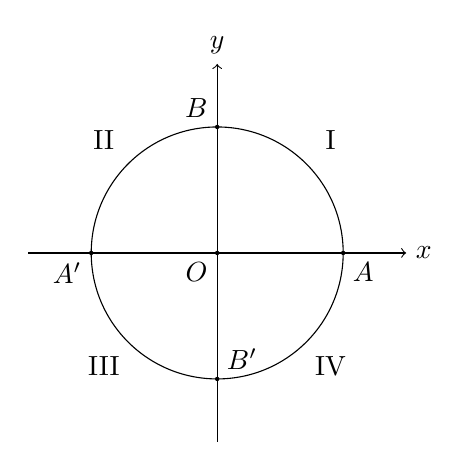
\begin{tikzpicture}[scale=0.8]
				\draw[->] (-3,0)  -- (3,0) node[right] {$x$};
				\draw[->] (0,-3)  -- (0,3) node[above] {$y$};
				\draw  (0,0) circle (2);
				 \coordinate (A) at (2,0);
				\coordinate (B) at  (0,2);
				 \coordinate (A') at (-2,0);
				\coordinate (B') at (0,-2); 
				\fill (A) circle (1pt) node[below right] {$A$}; 
				\fill (B) circle (1pt) node[above  left] {$B$};
				\fill (A') circle (1pt) node[below left] {$A'$}; 
				\fill (B') circle (1pt)  node[above right] {$B'$};
				 \node at (1.8,1.8) {I};
				\node  at (-1.8,1.8) {II};
				 \node at (-1.8,-1.8) {III};
				 \node at (1.8,-1.8) {IV};
				\fill (0,0) circle (1pt) node[below left]  {$O$};
			\end{tikzpicture}
		 }
	} 
\end{ex}

% từ: cau-hoi/lop11/1D1_Ham_so_luong_giac_va_phuong_trinh_luong/1D1-1-4_Do_dai_cua_mot_cung_tron.tex
\begin{ex}%[1D1N1-4]%[ma:2c4751b3]
	Cho $\dfrac{\pi}{2}<\alpha <\pi$. Kết quả đúng là 
	 \choice
		 {$\sin \alpha >0$, $\cos \alpha >0$}
		{$\sin  \alpha <0$, $\cos \alpha <0$}
		{\True  $\sin \alpha >0$, $\cos \alpha <0$}
		{$\sin \alpha <0$, $\cos  \alpha >0$}
	 \loigiai{
	Vì $\dfrac{\pi}{2}<\alpha <\pi$  nên $\sin \alpha >0$; $\cos \alpha <0$.}
\end{ex}

% từ: cau-hoi/lop11/1D1_Ham_so_luong_giac_va_phuong_trinh_luong/1D1-2-1_Cau_hoi_ly_thuyet.tex
\begin{ex}%[1D1Y2-1]%[ma:934609de]
	Nghiệm của phương trình $\cos \left(x+\dfrac{\pi }{3}\right)=0$ là 
	\choice 
		{ $ x=-\dfrac{\pi  }{3}+k\pi; ~k\in \mathbb{Z}$}
		{\True $  x=\dfrac{\pi }{6}+k2\pi; ~k\in \mathbb{Z}$}
		{ $  x=-\dfrac{5\pi }{6}+k2\pi; ~k\in \mathbb{Z}$}
		{ $ x=\dfrac{25\pi }{6}+k\pi; ~k\in \mathbb{Z}$} 
	 \loigiai{
		 Ta có $\cos \left(x+\dfrac{\pi }{3}\right)=0\Leftrightarrow x+\dfrac{\pi }{3}=\dfrac{\pi }{2}+k2\pi \Leftrightarrow x=\dfrac{\pi }{6}+k2\pi $, $ k\in \mathbb{Z}$.
	} 
\end{ex}

% từ: cau-hoi/lop11/1D1_Ham_so_luong_giac_va_phuong_trinh_luong/1D1-2-1_Cau_hoi_ly_thuyet.tex
\begin{ex}%[1D1Y2-1]%[ma:15754c25]
	Phương trình $ \sin \left(x-\dfrac{\pi}{3}\right)=1 $  có nghiệm là
	\choice 
		{$x=\dfrac{5\pi}{6}+k\pi, k\in \mathbb{Z} $} 
		 {$x=\dfrac{\pi}{3}+k2\pi, k\in \mathbb{Z} $}
		{\True $x=\dfrac{5\pi}{6}+k2\pi, k\in  \mathbb{Z} $}
		 {$x=\dfrac{\pi}{3}+k\pi, k\in \mathbb{Z} $}
	 \loigiai{
		Ta có: $\sin \left(x-\dfrac{\pi}{3}\right)=1\Leftrightarrow x-\dfrac{\pi}{3}=\dfrac{\pi}{2}+k2\pi, k\in \mathbb{Z}\Leftrightarrow x=\dfrac{5\pi}{6}+k2\pi, k \in  \mathbb{Z} $.
	 }
\end{ex}

% từ: cau-hoi/lop11/1D1_Ham_so_luong_giac_va_phuong_trinh_luong/1D1-5-3_Phuong_trinh_co_ban_dung_Radian.tex
\begin{ex}%[1D1H5-3]%[ma:841ffef8]
 Một nhà nghiên cứu ghi lại thời gian  (giờ) sử dụng Facbook của 30 học sinh trong 02 tuần.
 Kết quả thu được mẫu số liệu  như sau:
 \begin{center}
  \begin{tabular}{cccccccccc}
   21 & 17 &  22 & 18 & 20 & 17 & 15 & 13 & 15 & 20 \\
   15 & 12 & 18  & 17 & 25 & 17 & 21 & 15 & 12 & 18 \\
   16 & 23 & 14 & 18 & 19 & 13 & 16 & 19 & 18 & 17 
  \end{tabular}
 \end{center}
 \choiceTF 
  {Số giờ trung bình của học sinh trong 02 tuần là  $16{,}37$ giờ}
  {\True Tổng hợp kết quả thời gian sử dụng Facbook của học sinh vào bảng tần số ghép nhóm  theo mẫu sau\\
  \begin{tabular}{|c|c|c|c|c|c|}
   \hline 
   Số giờ & $[12;15)$ & $[15; 18)$  & $[18;21)$ & $[21; 24)$ & $[24;27)$ \\ \hline
   Giá trị đại diện  & $13{,}5$ & $16{,}5$ & $19{,}5$ & $22{,}5$ & $25{,}5$ \\ \hline
   Số học sinh & 5 & 12 & 8 & 4 & 1 \\ \hline 
 \end{tabular}}
 {\True Nhóm chứa mốt của mẫu số liệu ý b) là nhóm $[15; 18)$} 
 {\True Mốt của mẫu số liệu  ý b) bằng $16{,}91$}
 \loigiai{ 
  \begin{itemchoice}
   \itemch \textbf{Sai}. Tổng số thời gian sử dụng Facbook của 30 học  sinh là 521 giờ.\\
   Số giờ trung bình của học sinh trong  02 tuần là $\bar{x}=\frac{521}{30}=17{,}37$ giờ.
   \itemch \textbf{Đúng}. 
   \begin{center}
    \begin{tabular}{|c|c|c|c|c|c|}
     \hline 
     Số giờ & $[12;15)$  & $[15; 18)$ & $[18;21)$ & $[21; 24)$ & $[24;27)$ \\ \hline
     Giá trị đại diện &  $13{,}5$ & $16{,}5$ & $19{,}5$ & $22{,}5$ & $25{,}5$ \\ \hline
     Số học sinh & 5 & 12 & 8 & 4 & 1 \\ \hline 
    \end{tabular}
   \end{center}
   \itemch \textbf{Đúng}. Nhóm chứa mốt của mẫu số liệu trên là nhóm  $[15; 18)$.
    \itemch \textbf{Đúng}. Do đó, $u_m=15; n_{m-1}=5; n_m=12; n_{m+1}=8; u_{m+1}-u_m=18-15=3,0$.\\
   $M_{\circ}=15+\frac{12-5}{(12-5)+(12-8)} \cdot  3=16{,}91.$
  \end{itemchoice}
  }
\end{ex}

% từ: cau-hoi/lop11/1D1_Ham_so_luong_giac_va_phuong_trinh_luong/1D1-5-3_Phuong_trinh_co_ban_dung_Radian.tex
\begin{ex}%[1D1H5-3]%[ma:72e07f96]
 Thâm niên giảng dạy của một số giáo  viên trường THPT được ghi lại ở bảng sau
 \begin{center}
  \begin{tabular}{|c|c|c|c|c|c|}
    \hline
   Thâm niên (Số  năm) & $[1;5)$ & $[5; 10)$ & $[10;15)$ & $[15; 20)$ & $[20;25)$ \\ \hline
   Số giáo viên & 4  & 12 & 16 & 8 & 3 \\ \hline
  \end{tabular}
 \end{center}
 \choiceTF 
  {\True Cỡ mẫu của  mẫu số liệu bằng $50$}
  {\True Số trung  bình của mẫu ghép nhóm là $11{,}84$}
  {\True Nhóm  chứa mốt của mẫu số liệu trên là nhóm $[10; 15)$}
  {Mốt của  mẫu số liệu ghép nhóm bằng $11{,}74$}
  \loigiai{
  \begin{itemchoice}
   \itemch \textbf{Đúng}. Ta viết lại bảng tần số ghép nhóm theo giá  trị đại diện là
   \begin{center}
    \begin{tabular}{|c|c|c|c|c|c|}
     \hline 
     Thâm niên (Số năm) &  $[1;5)$ & $[5; 10)$ & $[10;15)$ & $[15; 20)$ & $[20;25)$ \\ \hline
     Giá trị đại diện & 3 &  $7{,}5$ & $12{,}5$ & $17{,}5$ & $22{,}5$ \\ \hline
     Số giáo viên & 4 & 12 & 16  & 8 & 3 \\ \hline
    \end{tabular}
   \end{center}
   Cỡ mẫu  của mẫu số liệu bằng $50$.
   \itemch \textbf{Đúng}.  Ước lượng số trung bình của mẫu ghép là
   $$\bar{x}=\dfrac{3\cdot4+7{,}5\cdot12+12{,}5\cdot16+17{,}5\cdot8+22{,}5\cdot3}{50}=11{,}84.$$ 
   \itemch  \textbf{Đúng}. Nhóm chứa mốt của mẫu số liệu trên là nhóm $[10; 15)$.
   \itemch \textbf{Sai}. Do  đó, $u_m=10, n_{m-1}=12, n_m=16, n_{m+1}=8, n_{m+1}-u_m=15-10=5$.
   $$M_{\circ}=10+\frac{16-12}{(16-12)+(16-8)} \cdot 5=11{,}66.$$ 
  \end{itemchoice}
 } 
\end{ex}

% từ: cau-hoi/lop11/1D2_Day_so_Cap_so_cong_Cap_so_nhan/1D2-2-6_Tinh_tong_cua_cap_so_cong.tex
\begin{ex}%[1D2H2-6]%[ma:dec7b287]
	Biết $\lim\limits_{x\to 3}\dfrac{x^2+bx+c}{x-3}=8$  ($b$, $c\in\mathbb{R}$). Tính $P=b+c$.
	\choice 
		{\True$P=-13$} 
		{$P=-11$} 
		{$P=5$} 
		{$P=-12$} 
	 \loigiai{
		Vì $\lim\limits_{x\to 3}\dfrac{x^2+bx+c}{x-3}=8$ là hữu  hạn nên tam thức $x^2+bx+c$ có nghiệm $x=3$ khi và chỉ khi $3b+c+9=0\Leftrightarrow c=-9-3b$.
		Khi đó 
		\begin{eqnarray*}
			& &\lim\limits_{x\to 3}\dfrac{x^2+bx+c}{x-3}\\ 
			&=&\lim\limits_{x\to  3}\dfrac{x^2+bx-9-3b}{x-3}\\
			&=&\lim\limits_{x\to 3} \dfrac{(x-3)(x+3+b)}{x-3}\\ 
			&=&\lim\limits_{x\to 3}  (x+3+b)=6+b.
		\end{eqnarray*}
		Suy ra  $6+b=8\Leftrightarrow b=2$ suy ra $c=-15$.\\
		Vậy  $P=b+c=-13$.
	 }
\end{ex}

% từ: cau-hoi/lop11/1D2_Day_so_Cap_so_cong_Cap_so_nhan/1D2-3-2_Nhan_dien_cap_so_nhan_cong_boi.tex
\begin{ex}%[1D2N3-2]%[ma:8a6d3fd9]
  Cho góc lượng giác $x$, biết $\tan x=\dfrac{1}{3}$ với $\dfrac{\pi}{2}<x<\pi$. Khi đó
 \choiceTF 
   {\True $\cos x<0$}
  {$\cos x=-\dfrac{\sqrt{10}}{10}$} 
  {\True  $\sin x=-\dfrac{\sqrt{10}}{10}$}
  {$\sin  x+\cos x=-\dfrac{\sqrt{10}}{5}$}
  \loigiai{
  \begin{itemchoice}
   \itemch Đúng. Ta có $\tan x=\frac{1}{3} \Rightarrow \cot x=\dfrac{1}{\tan x}=3$. Vì  $\dfrac{\pi}{2}<x<\pi$ nên $\cos x<0$.
   \itemch Sai. Ta có $\dfrac{1}{\cos ^2 x}=1+\tan ^2 x=1+\dfrac{1}{9}=\dfrac{10}{9} \Rightarrow \cos ^2 x=\dfrac{9}{10}  \Rightarrow \cos x=-\dfrac{3 \sqrt{10}}{10}$.
   \itemch  Đúng. $\sin x=\cos x \cdot\tan x=-\dfrac{3 \sqrt{10}}{10} \cdot \dfrac{1}{3}=-\dfrac{\sqrt{10}}{10}$ .
   \itemch Sai. $\sin  x+\cos x=-\dfrac{2 \sqrt{10}}{5}$.
  \end{itemchoice}
 } 
\end{ex}

% từ: cau-hoi/lop11/1D2_Day_so_Cap_so_cong_Cap_so_nhan/1D2-3-3_So_hang_tong_quat_cua_cap_so_nhan.tex
\begin{ex}%[1D2V3-3]%[ma:f36aa6b9]
	Cho dãy  số $(u_n)$ biết $\heva{&u_1=3\\&u_{n+1}=3u_n},\forall n\in \mathbb{N}^*$. Tìm số hạng tổng quát của dãy số $(u_n)$.
	\choice 
		{$u_n=n^{n+1}$} 
		{\True $u_n=3^n$} 
		{$u_n=3^{n+1}$} 
		 {$u_n=3^{n-1}$}
	\loigiai{ 
		Ta có $(u_n)$ là cấp số nhân với số hạng đầu $u_1=3$  và công bội $q=\dfrac{u_{n+1}}{u_n}=3$.\\
	 Do đó số hạng tổng quát $u_n=u_1\cdot q^{n-1}=3\cdot 3^{n-1}=3^n$.}
\end{ex}

% từ: cau-hoi/lop11/1D3_Gioi_han_Ham_so_lien_tuc/1D3-1-1_Cau_hoi_ly_thuyet.tex
\begin{ex}%[1D3N1-1]%[ma:f2f5a187]
	Trong các mệnh đề sau, mệnh đề nào là mệnh đề  \textbf{đúng}?
	\choice 
		 {$\lim\limits_{x\to+\infty} \dfrac{1}{n}=1$}
		{$\lim\limits_{x\to+\infty} q^n=0,  q>1$}
		 {$\lim\limits_{x\to+\infty} 1^n=0$}
		{\True  $\lim\limits_{x\to+\infty} q^n=0,|q|<1$}
	 \loigiai{Dựa vào một số giới hạn đặc biệt:
		$\lim\limits_{x\to+\infty}  \dfrac{1}{n}=0; \lim\limits_{x\to+\infty} q^n=0 , |q|<1$.
	} 
\end{ex}

% từ: cau-hoi/lop11/1D3_Gioi_han_Ham_so_lien_tuc/1D3-1-3_Phuong_phap_luong_lien_hop_lim_huu_han.tex
\begin{ex}%[1D3N1-3]%[ma:66cf17bc]
	Tính  $L = \lim\limits_{x\to 1} \dfrac{1-x}{\sqrt{2-x}-1}$.
	\choice 
		{$L  = -6$}
		{$L =  -4$}
		{\True $L =  2$}
		{$L =  -2$}
	 \loigiai{
		$L = \lim\limits_{x\to 1}  \dfrac{1-x}{\sqrt{2-x}-1}
		 = \lim\limits_{x\to 1} \dfrac{(1-x)(\sqrt{2-x}+1)}{-x+1}
		= \lim\limits_{x\to  1} (\sqrt{2-x}+1) = 2$.
	 }
\end{ex}

% từ: cau-hoi/lop11/1D3_Gioi_han_Ham_so_lien_tuc/1D3-1-5_Cap_so_nhan_lui_vo_han.tex
\begin{ex}%[1D3V1-5]%[ma:9d2f0664]
 Cho cấp số nhân lùi vô hạn $(u_n)$ có số hạng đầu bằng $2$ và công  bội bằng $\dfrac{1}{3}$.
 \choiceTF 
  {\True Số hạng thứ  hai của cấp số nhân là $u_2=\dfrac{2}{3}$}
  {Số  hạng thứ $5$ của cấp số nhân là $u_5=\dfrac{1}{81}$}
  {Tổng của $5$ số hạng đầu của cấp số nhân bằng  $\dfrac{242}{243}$}
  {\True Tổng  cấp số nhân lùi vô hạn $(u_n)$ bằng $3$}
 \loigiai{ 
 Ta  có $u_1 = 2$ và công bội $q = \dfrac{1}{3}$.
 \begin{itemchoice}
   \itemch $u_2=u_1\cdot q=2\cdot \dfrac{1}{3}=\dfrac{2}{3}$.
  \itemch  $u_5 = u_1q^4 = \dfrac{2}{3^4}= \dfrac{2}{81}$.
  \itemch Tổng của $5$ số hạng đầu của cấp số nhân là $S_5  = u_1\dfrac{1-q^5}{1-q} = 2\dfrac{1 - \left(\dfrac{1}{3}\right)^5}{1 - \dfrac{1}{3}} = 3\left[1 - \left(\dfrac{1}{3}\right)^5\right]=\dfrac{242}{81}$.
  \itemch Khi đó tổng của cấp số nhân lùi vô hạn đã  cho là
  $$S = \dfrac{u_1}{1-q} =\dfrac{2}{1-\dfrac{1}{3}}  =3.$$
 \end{itemchoice}
 } 
\end{ex}

% từ: cau-hoi/lop11/1D3_Gioi_han_Ham_so_lien_tuc/1D3-2-1_Cau_hoi_ly_thuyet.tex
\begin{ex}%[1D3B2-1]%[ma:97c6e599]
	Cho  dãy số $\left(u_n\right)$ biết $\heva{
	& u_1=2 \\ 
	& {u}_{n+1}=2u_n, \forall n  \in \mathbb{N}^{*}}$. Tìm số hạng tổng quát của dãy số này.
	 \choice
		{\True  $u_n=2^n$}
		 {$u_n={n}^{n-1}$}
		 {$u_n=2$}
		{$u_n={2}^{n+1}$} 
	 \loigiai{
	 Ta có
	$u_n=2{u}_{n-1}=2  \cdot 2{u}_{n-2}= \ldots ={2}^{n-1} \cdot u_1=2^n$.
	 }
\end{ex}

% từ: cau-hoi/lop11/1D3_Gioi_han_Ham_so_lien_tuc/1D3-2-1_Cau_hoi_ly_thuyet.tex
\begin{ex}%[1D3B2-1]%[ma:91eb9fdd]
	Cho dãy số  $(u_n)$ xác định bởi $ \heva{&u_1=2008 \\ &u_2=2009 \\ &2{{u}_{n+1}}=u_n+{{u}_{n+2}}\quad \text{ với } n\ge 1}$. Số hạng tổng quát của dãy là
	\choice 
		{\True $u_n=n+2007$} 
		{$u_n=2n+2006$} 
		 {$u_n=n-2007$}
		 {$u_n=-n+2008$}
	\loigiai{ 
		Ta có $  u_n-u_{n-1}=1\Rightarrow u_n=u_{n-1}+1$. Suy ra $$ u_n=(u_n-u_{n-1})+(u_{n-1}-u_{n-2})+\cdots +(u_2-u_1)+u_1=1+1+. . . +1+u_1=n-1+2008=n+2007.$$
	 }
\end{ex}

% từ: cau-hoi/lop11/1D3_Gioi_han_Ham_so_lien_tuc/1D3-2-1_Cau_hoi_ly_thuyet.tex
\begin{ex}%[1D3K2-1]%[ma:6a8da0a5]
	Cho dãy $(u_n)$ được xác  định bởi $\heva{&u_1 = 1 \\ &u_{n+1} = u_n + n^2}$. Số hạng tổng quát của dãy số là
	\choice 
		{$u_n  = 1 + \dfrac{n(2n+1)(n+1)}{6}$}
		{$u_n  = 1 + \dfrac{(n-1)n(2n+2)}{6}$}
		{\True $u_n = 1  + \dfrac{(n-1)n(2n-1)}{6}$}
		{Tất cả  đều sai}
	\loigiai{ 
		Từ $u_{n+1} = u_n + n^2$, ta  có
		\begin{align*}
			&u_1 =  1\\
			&u_2 =  u_1 + 1^2\\
			&\vdots\qquad\vdots\\ 
			&u_n = u_{n-1} + (n-1)^2. 
		\end{align*}
		Cộng vế theo vế ta được $u_n = 1 + 1^2 + 2^2 + \cdots  + (n-1)^2$.\\
		Mặt khác ta có $1^2 +  2^2 + 3^2 + \cdots + (n-1)^2 + n^2 = \dfrac{n(n+1)(2n+1)}{6}$\\
		 $\Rightarrow 1^2+2^2+3^2+ \cdots + (n-1)^2=\dfrac{n(n-1)(2n-1)}{6}$\\
		 Vậy $u_n=1+\dfrac{(n-1)n(2n-1)}{6}.$
	 }
\end{ex}

% từ: cau-hoi/lop11/1D3_Gioi_han_Ham_so_lien_tuc/1D3-2-1_Cau_hoi_ly_thuyet.tex
\begin{ex}%[1D3B2-1]%[ma:488a014a]
	Cho dãy số $(u_n)$ với $\heva{&u_1=1\\&u_{n+1}=u_n+(-1)^{2n}}$.  Số hạng tổng quát $u_n$ của dãy là
	 \choice
		{$u_n=2n-1$} 
		 {\True $u_n=n$}
		 {$u_n=n$}
		 {$u_n=n$}
	\loigiai{Ta có $u_{n+1}=u_n+(-1)^{2n}=u_n+1 \Rightarrow u_2=2;  u_3=3; u_3=4;...$ Dễ dàng đoán được $u_n=n$. \\
		Thật vậy, ta chứng minh được  $u_n=n\ (*)$ bằng phương pháp quy nạp như sau:
		 $(*)$ đúng khi $n=1$.\\
		Giả sử $(*)$ đúng với $n=k, k\in \mathbb{N}^*$ ta có $u_k=k$. Ta  đi chứng minh $(*)$ cũng đúng với $n=k+1$ tức là $u_{k+1}=k+1$. \\
	Thật vậy từ hệ thức  truy hồi ta có $u_{k+1}=u_k+(-1)^{2k}=k+1$ (đpcm). Vậy công thức số hạng tổng quát $u_n=n$.}
\end{ex}

% từ: cau-hoi/lop11/1D3_Gioi_han_Ham_so_lien_tuc/1D3-2-1_Cau_hoi_ly_thuyet.tex
\begin{ex}%[1D3B2-1]%[ma:acb6cb3c]
	Cho dãy số $(u_n)$ xác định bởi $ \heva{&u_1=1  \\ &u_n=2u_{n-1}+3\quad\forall n\ge 2 }$. Số hạng tổng quát của dãy là
	 \choice
		{\True  $u_n=2^{n+1}-3 $}
		{$u_n=2^{n+2}-7 $} 
		{$u_n=2^{n}-1 $} 
		{$u_n=2^{n-1}+1  $}
	\loigiai{Số hạng  tổng quát của dãy là $u_n=2^{n+1}-3 $. Ta chứng minh bằng phương pháp quy nạp
		\begin{itemize}
			\item  Với $ n=1\Rightarrow u_1=2^{1+1}-3=1\Rightarrow $ bài toán đúng với $ n=1 $.
			\item Giả sử $u_k=2^{k+1}-3  $, ta chứng minh $u_{k+1}=2^{k+2}-3 $.\\
			Thật vậy, theo  công thức truy hồi ta có $u_{k+1}=2u_k+3=2(2^{k+1}-3)+3=2^{k+2}-3 $.
		\end{itemize}
	 }
\end{ex}

% từ: cau-hoi/lop11/1D3_Gioi_han_Ham_so_lien_tuc/1D3-2-1_Cau_hoi_ly_thuyet.tex
\begin{ex}%[1D3B2-1]%[ma:edf4f288]
	Cho dãy số $(u_n)$ có $\heva{&u_1=3  \\&u_{n+1}=u_n+5 \text{ với }n\ge1}$. Số hạng tổng quát của dãy số là
	 \choice
		{$u_n=7n-4$} 
		{$u_n=4n-1$} 
		 {$u_n=n+2$}
		{\True $u_n=5n-2$} 
	 \loigiai{Ta có $u_2=8=5\cdot2-2, u_3=13=5\cdot3-2, u_4=18=5\cdot4-2 $.\\
	Dự đoán $\forall n\ge1$, ta có $u_n=5n-2$ $(1)$.\\ 
	Ta  chứng minh bằng phương pháp quy nạp.\\
	Với $n=1$, ta  có $u_1=3=5\cdot 1-2$. Vậy $(1)$ đúng với $n=1$.\\
	Giả sử $(1)$ đúng với  $n=k$ tức là ta có $u_k=5\cdot k-2$.\\
	Ta chứng minh $(1)$ cũng đúng với $n=k+1$,  tức là phải chứng minh
	$u_{k+1}=5.(k+1)-2$. \\ 
	Thật vậy, theo giả thiết quy nạp ta có $u_{k+1}=u_{k}+5=(5k-2)+5=5k+5-2=5(k+1)-2$.\\ 
	Vậy $(1)$ đúng với $n=k+1$  do đó $(1)$ đúng với mọi $n\ge1$.}
\end{ex}

% từ: cau-hoi/lop11/1D3_Gioi_han_Ham_so_lien_tuc/1D3-2-1_Cau_hoi_ly_thuyet.tex
\begin{bt}%[1D3Y2-1]%[ma:cc8169d3]
	Cho dãy số $(u_n)$  với các số hạng đầu là $5;10;15;20;25;\ldots$. Tìm số hạng tổng quát của dãy số này.
	\loigiai{Từ tính chất các số hạng của dãy suy ra số hạng tổng quát của dãy $(u_n)$  là $u_n=5n$.}
\end{bt}

% từ: cau-hoi/lop11/1D3_Gioi_han_Ham_so_lien_tuc/1D3-2-2_Thay_so_truc_tiep.tex
\begin{ex}%[1D3Y2-2]%[ma:bdc1f4f5]
	Cho dãy  số $({{u}_{n}}),$ biết ${{u}_{n}}={{(-1)}^{n}}\cdot \dfrac{{{2}^{n}}}{n}$. Tìm số hạng ${{u}_{3}}$.
	 \choice
		{  \True ${{u}_{3}}=-\dfrac{8}{3}$}
		{${{u}_{3}}=2$ } 
		 {${{u}_{3}}=-2$ }
		{${{u}_{3}}=\dfrac{8}{3}$ } 
	 \loigiai{
		Thay trực tiếp hoặc dùng chức  năng CALC:\\
	$${{u}_{3}}={{(-1)}^3}\cdot  \dfrac{{{2}^3}}{3}=-\dfrac{8}{3}.$$}
\end{ex}

% từ: cau-hoi/lop11/1D3_Gioi_han_Ham_so_lien_tuc/1D3-2-2_Thay_so_truc_tiep.tex
\begin{ex}%[1D3B2-2]%[ma:de8142a4]
	Cho dãy số $\left(a_n\right)$ có $a_n=-n^2+4n+11,\forall n\in \mathbb{N}^*$. Tìm số hạng  lớn nhất của dãy số $\left(a_n\right)$.
	 \choice
		 {$14$}
		 {\True $15$}
		 {$13$}
		{$12$} 
	\loigiai{ 
		 Ta có $a_n=-(n-2)^2+15\le 15,\forall n\ge 1.$ Dấu bằng xảy ra khi $n-2=0\Leftrightarrow n=2.$\\
	Vậy số hạng lớn nhất của dãy số là số hạng bằng 15} 
\end{ex}

% từ: cau-hoi/lop11/1D3_Gioi_han_Ham_so_lien_tuc/1D3-2-2_Thay_so_truc_tiep.tex
\begin{ex}%[1D3B2-2]%[ma:2dc3f422]
	Cho dãy số $\left(a_n\right)$ có $a_n=\dfrac{n}{n^2+100},\forall n\in \mathbb{N}^*$. Tìm số hạng lớn nhất của dãy số $\left(a_n\right)$. 
	\choice 
		 {\True $\dfrac{1}{20}$}
		{$\dfrac{1}{30}$} 
		 {$\dfrac{1}{25}$}
		{$\dfrac{1}{21}$} 
	\loigiai{ 
		Ta có $a_n=\dfrac{n}{n^2+100}\le \dfrac{n}{2\sqrt{n^2.100}}=\dfrac{1}{20}.$ Dấu  bằng xảy ra khi $n^2=100\Leftrightarrow n=10.$\\
	Vậy số hạng lớn nhất của dãy  là số hạng bằng $\dfrac{1}{20}$}
\end{ex}

% từ: cau-hoi/lop11/1D3_Gioi_han_Ham_so_lien_tuc/1D3-2-2_Thay_so_truc_tiep.tex
\begin{ex}%[1D3B2-2]%[ma:792553b2]
	Cho dãy số $(u_n)$ có số hạng tổng quát $u_n=\dfrac{2n+1}{n+2}$. Số $\dfrac{167}{84}$  là số hạng thứ mấy?
	 \choice
		{300} 
		 {212}
		 {\True 250}
		{249} 
	 \loigiai{
		Giả sử $u_n=\dfrac{167}{84}\Rightarrow  \dfrac{2n+1}{n+2}=\dfrac{167}{84}\Leftrightarrow 84(2n+1)=167(n+2)$$\Leftrightarrow n=250$.\\
	Vậy $\dfrac{167}{84}$ là số hạng thứ $250$  của dãy số $(u_n)$.}
\end{ex}

% từ: cau-hoi/lop11/1D3_Gioi_han_Ham_so_lien_tuc/1D3-2-2_Thay_so_truc_tiep.tex
\begin{ex}%[1D3B2-2]%[ma:1a355848]
	Cho dãy số $(u_n)$ có số hạng tổng quát:  $u_n = 2n+\sqrt{n^2+4}$. Dãy số đã cho có bao nhiêu số hạng là số nguyên.
	 \choice
		 {$1$}
		 {$2$}
		{$3$} 
		{\True$0$} 
	 \loigiai{
		Ta  có $u_n$ nguyên $\Leftrightarrow \sqrt{n^2+4}=k\in\mathbb{N} \Leftrightarrow k^2-n^2=4 \Leftrightarrow (k-n)(k+n)=4$. Phương trình này vô nghiệm.\\
	Vậy  không có số hạng nào của dãy nhận giá trị nguyên.}
\end{ex}

% từ: cau-hoi/lop11/1D3_Gioi_han_Ham_so_lien_tuc/1D3-2-2_Thay_so_truc_tiep.tex
\begin{ex}%[1D3B2-2]%[ma:be484a39]
	Cho dãy số có 4 số hạng đầu là $-1,3,19,53$. Hãy tìm một quy luật của dãy số trên và viết số hạng thứ 10 của dãy với quy luật  vừa tìm.
	\choice 
		{$u_{10}=97$} 
		 {$u_{10}=71$}
		 {$u_{10}=1414$}
		 {\True $u_{10}=971$}
	 \loigiai{
		Xét dãy $(u_n)$ có dạng: $u_n=an^3+bn^2+cn+d$.\\ 
		Ta  có hệ $\heva{
		&  a+b+c+d=-1 \\
		&  8a+4b+2c+d=3 \\
		& 27a+9b+3c+d=19 \\ 
		 & 64a+16b+4c+d=53. \\}$\\
		Giải hệ trên ta tìm được: $a=1,b=0,c=-3,d=1$$\Rightarrow  u_n=n^3-3n+1$ là một quy luật.\\
	Số hạng thứ 10: $u_{10}=971$.} 
\end{ex}

% từ: cau-hoi/lop11/1D3_Gioi_han_Ham_so_lien_tuc/1D3-2-2_Thay_so_truc_tiep.tex
\begin{ex}%[1D3B2-2]%[ma:230aaa7b]
	Cho dãy số $(u_n)$ được xác định bởi $u_n=\dfrac{n^2+3n+7}{n+1}$. 
	Dãy số có bao  nhiêu số hạng nhận giá trị nguyên.
	 \choice
		{$2$} 
		 {$4$}
		{\True $1$} 
		 {Không có}
	 \loigiai{
		Ta có $u_n=n+2+\dfrac{5}{n+1}$, do đó $u_n$ nguyên khi và chỉ khi $\dfrac{5}{n+1}$ nguyên hay $n+1$ là ước của $5$. \\ 
		Điều đó xảy ra  khi $n+1=5\Leftrightarrow n=4$.\\
	Vậy dãy số có  duy nhất một số hạng nguyên là $u_4=7$}
\end{ex}

% từ: cau-hoi/lop11/1D3_Gioi_han_Ham_so_lien_tuc/1D3-2-2_Thay_so_truc_tiep.tex
\begin{ex}%[1D3K2-2]%[ma:6ffb1beb]
	Cho dãy số $(a_n)$ xác định bởi $a_1=-3$ và  $a_{n + 1}=a_n + n^2 - 3n + 4,\forall n\in\mathbb{N}^{*}$. Số $1391$ là số hạng thứ mấy của dãy số đã cho?
	\choice 
		 {\True$18$}
		{$17$} 
		{$20$} 
		 {$19$}
	 \loigiai{
	Từ hệ thức truy hồi của  dãy số $(a_n)$ ta có
	 $$
	a_n=a_1 + \left[1^2  + 2^2 + \ldots + (n - 1)^2\right] - 3[1 + 2 + \ldots + (n - 1)] + 4(n - 1)\Leftrightarrow a_n=\dfrac{n^3 - 6n^2 + 17n - 21}{3}.$$
	Suy ra số hạng tổng quát của dãy số  $(a_n)$ là $a_n=\dfrac{n^3 - 6n^2 + 17n - 21}{3}$.
	 Giải phương trình $a_n=1391$ ta được $n=18$.
	 }
\end{ex}

% từ: cau-hoi/lop11/1D3_Gioi_han_Ham_so_lien_tuc/1D3-2-2_Thay_so_truc_tiep.tex
\begin{ex}%[1D3B2-2]%[ma:c0a61f1a]
	Cho dãy số $\left(y_n\right)$ xác định bởi $y_1=2$ và ${y}_{n+1}=2y_n+n^2-3n,\forall n\in \mathbb{N}^*$. Tổng $S_4$ của $4$  số hạng đầu tiên của dãy số là:
	 \choice
		 {\True $S_4=20$}
		 {$S_4=10$}
		{$S_4=30$} 
		{$S_4=14$} 
	\loigiai{ 
	 Ta tính được $y_2=2;y_3=4;y_4=12\Rightarrow S_4=20.$}
\end{ex}

% từ: cau-hoi/lop11/1D3_Gioi_han_Ham_so_lien_tuc/1D3-2-2_Thay_so_truc_tiep.tex
\begin{bt}%[1D3Y2-2]%[ma:3e18c3a3]
	Cho dãy số $(u_n)$ có  số hạng tổng quát $u_n=\dfrac{2n+1}{n+2}$. Viết năm số hạng đầu của dãy số.
	\loigiai{ 
	Năm số hạng đầu của  dãy là\\ $u_1=1,u_2=\dfrac{5}{4},u_3=\dfrac{7}{5},u_4=\dfrac{3}{2},u_5=\dfrac{11}{7}$.}
\end{bt}

% từ: cau-hoi/lop11/1D3_Gioi_han_Ham_so_lien_tuc/1D3-2-2_Thay_so_truc_tiep.tex
\begin{ex}%[1D3Y2-2]%[ma:b001bff3]
	Cho dãy số $(u_n)$ có số hạng tổng quát $u_n=\dfrac{2n+1}{n+2}$. Viết  năm số hạng đầu của dãy số.
	 \loigiai{
	 Năm số hạng đầu của dãy là\\ $u_1=1,u_2=\dfrac{5}{4},u_3=\dfrac{7}{5},u_4=\dfrac{3}{2},u_5=\dfrac{11}{7}$.}
\end{ex}

% từ: cau-hoi/lop11/1D3_Gioi_han_Ham_so_lien_tuc/1D3-2-2_Thay_so_truc_tiep.tex
\begin{ex}%[1D3Y2-2]%[ma:55a810c0]
	Cho dãy số $(a_n)$  xác định bởi: $\heva{
	& u_1=-1,u_2=3 \\ 
	& {u}_{n+1}=5u_n-6{u}_{n-1} \forall n\ge 2 \\}$. Viết 7 số hạng đầu tiên của  dãy số.
	\loigiai{ 
		Bảy  số hạng đầu của dãy là\\
		 $u_3=5u_2-6u_1=21$; $u_4=5u_3-6u_2=87$; $u_5=5u_4-6u_3=309$
	$u_6=5u_5-6u_4=1023$; $u_7=5u_6-6u_5=3261$} 
\end{ex}

% từ: cau-hoi/lop11/1D3_Gioi_han_Ham_so_lien_tuc/1D3-2-2_Thay_so_truc_tiep.tex
\begin{ex}%[1D3Y2-2]%[ma:8ddc606a]
	Cho  dãy số $(u_n)$ xác định bởi $\heva{
	 & u_1=1 \\
	& u_n=2{u}_{n-1}+3 \forall n\ge 2 \\}$. Viết năm số hạng đầu của  dãy số.
	\loigiai{ 
		Ta có 5 số  hạng đầu của dãy là\\
	$u_1=1$; $u_2=2u_1+3=5$; $u_3=2u_2+3=13$; $  u_4=2u_3+3=29$, $u_5=2u_4+3=61$.}
\end{ex}

% từ: cau-hoi/lop11/1D3_Gioi_han_Ham_so_lien_tuc/1D3-2-2_Thay_so_truc_tiep.tex
\begin{ex}%[1D3Y2-2]%[ma:3967e915]
	Cho dãy số  $(u_n):\heva{&u_1=u_2=1\\&u_n=u_{n-1}+u_{n-2}, \forall n\geq 3}$. Tìm số hạng thứ $7$ của dãy.
	 \loigiai{
		Ta  có $u_3=u_1+u_2=2, u_4=u_2+u_3=3, u_5=u_3+u_4=5, u_6=u_4+u_5=8, u_7=u_5+u_6=13$.
	} 
\end{ex}

% từ: cau-hoi/lop11/1D3_Gioi_han_Ham_so_lien_tuc/1D3-2-3_PP_dat_thua_so_chung_ket_qua_huu_han.tex
\begin{ex}%[1D3B2-3]%[ma:e616416d]
	 Cho dãy số $( u_n)$ với $u_n=2n-1$. Dãy số $( u_n)$ là dãy số
	 \choice
		{ Bị chặn  trên bởi 1}
		{  Giảm}
		{ Bị chặn dưới  bởi 2}
		{ \True Tăng} 
	 \loigiai{
	 $\forall n\in {{\mathbb{N}}^{*}}$ ta có ${{u}_{n+1}}-u_n=2( n+1)-1-( 2n-1)=2>0$ nên ${{u}_{n+1}}>u_n$.\\ Vậy dãy số $( u_n)$ tăng.}
\end{ex}

% từ: cau-hoi/lop11/1D3_Gioi_han_Ham_so_lien_tuc/1D3-2-3_PP_dat_thua_so_chung_ket_qua_huu_han.tex
\begin{ex}%[1D3B2-3]%[ma:fdb8ca11]
	Cho dãy số $( u_n)$ có $u_n=-{{n}^2}+n+1$. Khẳng định nào  sau đây là đúng?
	\choice 
		{ 5  số hạng đầu của dãy là: $-1;1;5;-5;-11;-19$}
		 { ${{u}_{n+1}}=-{{n}^2}+n+2$}
		 { ${{u}_{n-1}}-u_n=1$}
		{ \True Là một  dãy số giảm}
	\loigiai{ 
		Ta có\\ 
	${{u}_{n+1}}-u_n=[-{{(  n+1)}^2}+n+1+1]-[-{{n}^2}+n+1]\\=-{{n}^2}-2n-1+n+2+{{n}^2}-n-1=-2n<0$ $\forall n\ge 1$.\\ Do đó $( u_n)$ là một dãy giảm.}
\end{ex}

% từ: cau-hoi/lop11/1D3_Gioi_han_Ham_so_lien_tuc/1D3-2-3_PP_dat_thua_so_chung_ket_qua_huu_han.tex
\begin{ex}%[1D3B2-3]%[ma:8a5e7403]
	Trong các dãy số sau, dãy số nào là dãy số giảm 
	\choice 
		{ $u_n=\dfrac{n-3}{n+1}$} 
		{ $u_n=\dfrac{n}{2}$} 
		{ \True  $u_n=\dfrac{2}{{{n}^2}}$}
		 { $u_n=\dfrac{{{( -1)}^{n}}}{{{3}^{n}}}$}
	 \loigiai{
		Xét $u_n=\dfrac{n-3}{n+1};$ ${{u}_{n+1}}=\dfrac{n-2}{n+2}$. Khi đó:  ${{u}_{n+1}}-u_n=\dfrac{n-2}{n+2}-\dfrac{n-3}{n+1}=\dfrac{4}{( n+1)( n+2)}>0$ $\forall n\in \mathbb{N}^*$
		Vậy $( u_n)$ là dãy  số tăng.\\
		Xét $u_n=\dfrac{n}{2};$ ${{u}_{n+1}}=\dfrac{n+1}{2}$. Khi đó: ${{u}_{n+1}}-u_n=\dfrac{n+1}{2}-\dfrac{n}{2}=\dfrac{1}{2}>0$ $\forall n\in \mathbb{N}^*$. 
		Vậy $( u_n)$ là dãy số tăng.\\ 
		Xét $u_n=\dfrac{2}{{{n}^2}}$, ${{u}_{n+1}}=\dfrac{2}{{{( n+1)}^2}}$. $\dfrac{{{u}_{n+1}}}{u_n}=\dfrac{{{n}^2}}{{{( n+1)}^2}}<\dfrac{{{n}^2}}{{{n}^2}}=1,\forall n\in {{\mathbb{N}}^{*}}$. Vậy $( u_n)$  là dãy giảm.\\
	Xét ${{u}_{1}}=\dfrac{-1}{3};$ ${{u}_{2}}=\dfrac{1}{9};$ ${{u}_{3}}=\dfrac{-1}{27}$. Vậy $( u_n)$ là dãy  số không tăng không giảm}
\end{ex}

% từ: cau-hoi/lop11/1D3_Gioi_han_Ham_so_lien_tuc/1D3-2-3_PP_dat_thua_so_chung_ket_qua_huu_han.tex
\begin{ex}%[1D3B2-3]%[ma:b4469b4b]
	Trong các dãy số sau, dãy số  nào là dãy số giảm?
	 \choice
		{  \True $u_n=\dfrac{2n+1}{n-1}$}
		 { $u_n={{n}^3}-1$}
		{  $u_n={{n}^2}$}
		 { $u_n=2n$}
	 \loigiai{
		Với  mọi $n\in \mathbb{N}$, $n>1$. Ta có\\
		${{u}_{n+1}}-u_n=\dfrac{2( n+1)+1}{( n+1)-1}-\dfrac{2n+1}{n-1}=\dfrac{2n+3}{n}-\dfrac{2n+1}{n-1}$ 
		$=\dfrac{( 2n+3)( n-1)-n( 2n+1)}{n( n-1)}\\=\dfrac{( 2n+3)( n-1)-n( 2n+1)}{n( n-1)}=\dfrac{-3}{n(  n-1)}<0$, với mọi $n\in \mathbb{N}$, $n>1$.\\
	Suy  ra dãy số giảm.}
\end{ex}

% từ: cau-hoi/lop11/1D3_Gioi_han_Ham_so_lien_tuc/1D3-2-3_PP_dat_thua_so_chung_ket_qua_huu_han.tex
\begin{ex}%[1D3B2-3]%[ma:f6f7bfc2]
	Cho dãy  số $( u_n)$ với $u_n=\dfrac{{{(-1)}^{n-1}}}{n+1}$. Khẳng định nào sau đây là sai?
	 \choice
		{Số hạng thứ $9$ của dãy số là  $\dfrac{1}{10}$}
		{Số hạng thứ 10 của dãy số là $\dfrac{-1}{11}$} 
		{\True Đây là một dãy số giảm} 
		{Bị chặn trên bởi số $M=1$} 
	\loigiai{ 
	Dãy $u_n$ là một dãy đan dấu  nên khẳng định dãy giảm là sai.}
\end{ex}

% từ: cau-hoi/lop11/1D3_Gioi_han_Ham_so_lien_tuc/1D3-2-3_PP_dat_thua_so_chung_ket_qua_huu_han.tex
\begin{ex}%[1D3B2-3]%[ma:44ce4150]
	Cho dãy số $( u_n)$ với $u_n=\dfrac{1}{{{n}^2}+n}$. Khẳng định nào sau đây là sai? 
	 \choice
		 { $5$ số hạng đầu của dãy là:$\dfrac{1}{2};\dfrac{1}{6};\dfrac{1}{12};\dfrac{1}{20};\dfrac{1}{30}$}
		{ \True Là  dãy số tăng}
		{ Bị chặn trên bởi số $M=\dfrac{1}{2}$} 
		{ Không bị  chặn}
	\loigiai{ 
		Ta có\\ ${{u}_{n+1}}-u_n=\dfrac{1}{{{( n+1)}^2}+( n+1)}-\dfrac{1}{{{n}^2}+n}\\=\dfrac{1}{( n+1)( n+2)}-\dfrac{1}{n(  n+1)}$
		$=\dfrac{-2}{n( n+1)( n+2)}<0$ với  $n\ge 1$.
	Do đó $(  u_n)$ là dãy giảm.}
\end{ex}

% từ: cau-hoi/lop11/1D3_Gioi_han_Ham_so_lien_tuc/1D3-2-3_PP_dat_thua_so_chung_ket_qua_huu_han.tex
\begin{bt}%[1D3Y2-3]%[ma:21dda78a]
	Cho dãy số $( u_n)$  với $u_n=\sin n$. Xét tính tăng giảm của dãy số.
	 \loigiai{
	Ta có $\sin 1 < \sin 2$ nhưng $\sin 2 > \sin 3$ nên $u_n$ không tăng không giảm.  }
\end{bt}

% từ: cau-hoi/lop11/1D3_Gioi_han_Ham_so_lien_tuc/1D3-2-3_PP_dat_thua_so_chung_ket_qua_huu_han.tex
\begin{bt}%[1D3Y2-3]%[ma:781965a3]
	Cho dãy  số $( u_n)$ với $u_n=\dfrac{1}{n+1}$. Xét tính tăng giảm của dãy số.
	\loigiai{ 
	Ta có ${u}_{n+1}-{u}_{n}=\dfrac{1}{n+2}-\dfrac{1}{n+1}=\dfrac{n+1-n-2}{\left( n+2 \right)\left( n+1 \right)}=\dfrac{-1}{\left(  n+2 \right)\left( n+1 \right)}<0,\forall n\in {{\mathbb{N}}^{*}}$\\ Vậy ${u}_{n}$ là dãy giảm}
\end{bt}

% từ: cau-hoi/lop11/1D3_Gioi_han_Ham_so_lien_tuc/1D3-2-3_PP_dat_thua_so_chung_ket_qua_huu_han.tex
\begin{bt}%[1D3Y2-3]%[ma:a8175aca]
	Cho dãy số $( u_n)$ với $u_n={{n}^2}+1$.  Xét tính tăng giảm của dãy số.
	\loigiai{ 
	Ta có $u_{n+1}-u_{n}=\left(n+1\right)^2+1-n^2-1=2n+1>0, \forall n\in {{\mathbb{N}}^{*}}$.\\  Vậy $u_n$ là dãy tăng.}
\end{bt}

% từ: cau-hoi/lop11/1D3_Gioi_han_Ham_so_lien_tuc/1D3-2-3_PP_dat_thua_so_chung_ket_qua_huu_han.tex
\begin{ex}%[1D3Y2-3]%[ma:f60be9b1]
	Cho dãy số $( u_n)$ với $u_n=\sin n$. Xét  tính tăng giảm của dãy số.
	 \loigiai{
	Ta có $\sin 1 < \sin 2$ nhưng $\sin 2  > \sin 3$ nên $u_n$ không tăng không giảm. }
\end{ex}

% từ: cau-hoi/lop11/1D3_Gioi_han_Ham_so_lien_tuc/1D3-2-3_PP_dat_thua_so_chung_ket_qua_huu_han.tex
\begin{ex}%[1D3Y2-3]%[ma:dd9df834]
	Cho dãy số $( u_n)$ với $u_n=\dfrac{1}{n+1}$. Xét tính tăng  giảm của dãy số.
	 \loigiai{
	Ta có ${u}_{n+1}-{u}_{n}=\dfrac{1}{n+2}-\dfrac{1}{n+1}=\dfrac{n+1-n-2}{\left( n+2 \right)\left( n+1 \right)}=\dfrac{-1}{\left( n+2 \right)\left( n+1  \right)}<0,\forall n\in {{\mathbb{N}}^{*}}$\\ Vậy ${u}_{n}$ là dãy giảm}
\end{ex}

% từ: cau-hoi/lop11/1D3_Gioi_han_Ham_so_lien_tuc/1D3-2-4_PP_dat_thua_so_chung_ket_qua_vo_cuc.tex
\begin{ex}%[1D3H2-4]%[ma:b62bcd56]
	Một cấp số nhân có hai số hạng liên  tiếp là $16$ và $36$. Số hạng tiếp theo là
	\choice 
		{$720$} 
		{\True  $81$}
		 {$64$}
		 {$56$}
	\loigiai{ 
		Ta có cấp số nhân $\left(u_n\right)$ có 
		$ 
		\heva{ 
		& u_k=16  \\
		 & u_{k+1}=36
		} \Rightarrow q=\dfrac{u_{k+1}}{u_k}=\dfrac{9}{4}  \Rightarrow u_{k+2}=u_{k+1} q=81
		$. 
	} 
\end{ex}

% từ: cau-hoi/lop11/1D3_Gioi_han_Ham_so_lien_tuc/1D3-2-4_PP_dat_thua_so_chung_ket_qua_vo_cuc.tex
\begin{ex}%[1D3B2-4]%[ma:eee24862]
	Xét tính  tăng, giảm và bị chặn của dãy số $(u_n)$, biết $u_n=\dfrac{1}{\sqrt{1+n+n^2}}$
	 \choice
		 {Dãy số tăng, bị chặn trên}
		{Dãy số tăng,  bị chặn dưới}
		{\True  Dãy số giảm, bị chặn}
		{Dãy số không  bị chặn }
	 \loigiai{
		Ta  có $u_n>0, \,\forall n\in \mathbb{N}^*$ \\
		$\dfrac{u_{n+1}}{u_n}=\dfrac{\sqrt{n^2+n+1}}{\sqrt{(n+1)^2+(n+1)+1}}=\sqrt{\dfrac{n^2+n+1}{n^2+3n+3}}<1, \,\forall n \in  \mathbb{N}^*$.\\
		$ \Rightarrow  u_{n+1}<u_n, \,\forall n \in \mathbb{N}^* \Rightarrow $ dãy $(u_n)$ là dãy số giảm. \\
	Mặt khác $0<u_n<1 \Rightarrow $  dãy $(u_n)$ là dãy bị chặn.}
\end{ex}

% từ: cau-hoi/lop11/1D3_Gioi_han_Ham_so_lien_tuc/1D3-2-4_PP_dat_thua_so_chung_ket_qua_vo_cuc.tex
\begin{ex}%[1D3B2-4]%[ma:9efac565]
	Cho dãy số $(u_n)$, biết $u_n=\dfrac{2^n}{n!}$. Khẳng định nào  sau đây \textbf{đúng}?
	\choice 
		{Dãy số tăng, bị  chặn trên}
		{Dãy  số tăng, bị chặn dưới}
		{ \True Dãy số giảm, bị chặn trên} 
		{Dãy số giảm, bị chặn dưới} 
	 \loigiai{
		 Ta có $\dfrac{u_{n+1}}{u_n}=\dfrac{2^{n+1}}{(n+1)!} \colon \dfrac{2^n}{n!}=\dfrac{2^{n+1}}{(n+1)!}.\dfrac{n!}{2^n}=\dfrac{2}{n+1}<1, \forall n \in \mathbb{N}^*$ \\
		 Mà $\forall n \in \mathbb{N}^*, u_n>0, \Rightarrow u_{n+1}<u_n \Rightarrow $ dãy $(u_n)$ là dãy số giảm. \\
	Vì $0<u_n \leq u_1=2, \,\forall n \geq 1 \Rightarrow $ dãy $(u_n)$  là dãy bị chặn.}
\end{ex}

% từ: cau-hoi/lop11/1D3_Gioi_han_Ham_so_lien_tuc/1D3-2-4_PP_dat_thua_so_chung_ket_qua_vo_cuc.tex
\begin{bt}%[1D3B2-4]%[ma:7ee7a10f]
	Xét tính tăng, giảm và bị chặn của dãy số $(u_n)$, biết: $u_n=\dfrac{n^2+3n+1}{n+1}$. 
	\loigiai{ 
	Ta có $\forall n \in \mathbb{N}^*, u_n>\dfrac{n^2+2n+1}{n+1}=n+1 \geq 2  \Rightarrow $ dãy $(u_n)$ bị chặn dưới.}
\end{bt}

% từ: cau-hoi/lop11/1D3_Gioi_han_Ham_so_lien_tuc/1D3-2-4_PP_dat_thua_so_chung_ket_qua_vo_cuc.tex
\begin{ex}%[1D3Y2-4]%[ma:2689acdf]
	Cho dãy số $(u_n)$, biết: $1 \le u_n\le 10, \forall n\in \mathbb{N}^*$. Xét tính bị chặn của dãy số. 
	 \loigiai{
	Vì $1 \le u_n\le 10, \forall n\in \mathbb{N}^*$ nên giá trị lớn nhất của dãy số là $1$, giá trị lớn nhất của dãy số là  $10$.}
\end{ex}

% từ: cau-hoi/lop11/1D3_Gioi_han_Ham_so_lien_tuc/1D3-2-4_PP_dat_thua_so_chung_ket_qua_vo_cuc.tex
\begin{ex}%[1D3B2-4]%[ma:70d8c7c7]
	Xét tính  tăng, giảm và bị chặn của dãy số $(u_n)$, biết: $u_n=\dfrac{n^2+3n+1}{n+1}$.
	 \loigiai{
	Ta có $\forall n \in \mathbb{N}^*, u_n>\dfrac{n^2+2n+1}{n+1}=n+1 \geq 2 \Rightarrow  $ dãy $(u_n)$ bị chặn dưới.}
\end{ex}

% từ: cau-hoi/lop11/1D3_Gioi_han_Ham_so_lien_tuc/1D3-3-2_Tinh_lien_tuc_the_hien_qua_do_thi.tex
\begin{ex}%[1D3N3-2]%[ma:19edd384]
	\immini{ Hàm số $f(x)$ có đồ thị như hình bên  dưới không liên tục tại điểm có hoành độ là bao nhiêu?
	 \choice
		 {$x=0$}
		 {\True $x=1$}
		 {$x=2$}
		{$x=3$}}{\begin{tikzpicture}[scale=0.8,font=\footnotesize,line join=round,line cap=round,>=stealth]
		\draw[->]  (-2.1,0)--(5.1,0) node[below left] {$x$};
		\draw[->]  (0,-1.1)--(0,5.1) node[below left] {$y$};
		\draw (0,0)  node [below left] {$O$};
		\foreach  \x/\nx in {1/1,2/2}
		\draw[thin] (\x,1pt)--(\x,-1pt)  node [below] {$\nx$};
		 \foreach \y/\ny in {1/1,3/3}
		\draw[thin] (1pt,\y)--(-1pt,\y) node [left] {$\ny$}; 
		 \draw[dashed](1,0)--(1,3)--(0,3);
		\draw[dashed](2,0)--(2,1)--(0,1); 
		\begin{scope}
			\clip (-2,-1)  rectangle (5,5);
			\draw[samples=200,domain=1:-2,smooth,variable=\x] plot  (\x,{2*(\x)^2+1});
			\draw[samples=200,domain=5:1,smooth,variable=\x] plot  (\x,{(\x)-1});
		\end{scope}
	\end{tikzpicture}
		 }
	 \loigiai{
		Dựa vào đồ thị, ta thấy $\heva{&\lim\limits_{x\to 1^+}f(x)=0\\&\lim\limits_{x\to 1^-}f(x)=3}$  nên hàm số $f(x)$ gián đoạn tại $x=1$.
	 }
\end{ex}

% từ: cau-hoi/lop11/1D3_Gioi_han_Ham_so_lien_tuc/1D3-3-2_Tinh_lien_tuc_the_hien_qua_do_thi.tex
\begin{ex}%[1D3B3-2]%[ma:6355112c]
	Một cấp số cộng có $6$ số hạng. Biết rằng tổng của số hạng đầu và số hạng cuối bằng $17;$ tổng của số hạng thứ hai và số hạng thứ  tư bằng $14$. Tìm công sai $d$ của câp số cộng đã cho.
	\choice 
		{ $d=2$ } 
		{ $d=5$ } 
		{ \True $d=-3$ } 
		 { $d=4$ }
	 \loigiai{Ta có
		 $\heva{
		& {{u}_{1}}+{{u}_{6}}=17  \\
		 & {{u}_{2}}+{{u}_{4}}=14 \\
		}\Leftrightarrow  \heva{
		 & 2{{u}_{1}}+5d=17 \\
		&  2{{u}_{1}}+6d=14 \\
		 }\Leftrightarrow \heva{
		& {{u}_{1}}=16  \\
		& d=-3.  \\
	}$} 
\end{ex}

% từ: cau-hoi/lop11/1D3_Gioi_han_Ham_so_lien_tuc/1D3-3-3_Ham_so_lien_tuc_tai_mot_diem.tex
\begin{ex}%[1D3V3-3]%[ma:713e7d27]
	Cho hàm số $  f(x)=x^2-3x+2$.
	\choiceTF 
		{\True $\lim\limits_{x\to  1}\dfrac{f(x)}{x-1}=-1$}
		{$\lim\limits_{x\to 1}\dfrac{f(x)}{x^2-1}=\dfrac14$} 
		{$\lim\limits_{x\to  1}\dfrac{f(x)}{x^3-x^2+x-1}>0$}
		{\True Để $\lim\limits_{x\to 1}\dfrac{f(x)}{ax+b}=2$  thì $ a+3b=1$}
	\loigiai{\begin{itemchoice}
		\itemch $\lim\limits_{x\to 1}\dfrac{f(x)}{x-1}=\lim\limits_{x\to  1}\dfrac{x^2-3x+2}{x-1}=\lim\limits_{x\to 1}\dfrac{\left(x-2\right)\left(x-1\right)}{x-1}=\lim\limits_{x\to 1}\left(x-2\right)=-1$.
		\itemch  $\lim\limits_{x\to 1}\dfrac{f(x)}{x^2-1}=\lim\limits_{x\to 1}\dfrac{\left(x-2\right)\left(x-1\right)}{\left(x-1\right)\left(x+1\right)}=\lim\limits_{x\to 1}\dfrac{x-2}{x+1}=-\dfrac12$.
		\itemch $\lim\limits_{x\to 1}\dfrac{f(x)}{x^3-x^2+x-1}=\lim\limits_{x\to 1}\dfrac{\left(x-2\right)\left(x-1\right)}{\left(x-1\right)\left(x^2+1\right)}=\lim\limits_{x\to  1}\dfrac{x-2}{x^2+1}=-\dfrac12<0$.
		\itemch Để $\lim\limits_{x\to 1}\dfrac{f(x)}{ax+b}=2$  thì $ ax+b$ có nghiệm bằng $1\Leftrightarrow a+b=0\Leftrightarrow b=-a$.\\
		Khi đó $\lim\limits_{x\to 1}\dfrac{f(x)}{ax+b}=\lim\limits_{x\to 1}\dfrac{\left(x-2\right)\left(x-1\right)}{a\left(x-1\right)}=\lim\limits_{x\to 1}\dfrac{x-2}a=-\dfrac1a=2\Leftrightarrow a=-\dfrac12.$\\ 
		Từ  đó suy ra $b=-a=\dfrac12$.\\
		 Vậy, $ a+3b=-\dfrac12+3\cdot\dfrac12=1$.
\end{itemchoice}}
\end{ex}

% từ: cau-hoi/lop11/1D3_Gioi_han_Ham_so_lien_tuc/1D3-3-4_Ham_so_lien_tuc_tren_khoang_doan.tex
\begin{ex}%[1D3K3-4]%[ma:7b20d66d]
	Nếu $a;b;c$ theo thứ tự lập thành cấp số cộng thì dãy số nào sau  đây lập thành cấp số cộng?
	\choice 
		{  $2b;a;c$ }
		{  \True $-2b;-2a;-2c$ }
		{ $2b;-a;-c$} 
		{ $2b^2;a^2;{{c}^2}$  }
	 \loigiai{
	 Ta có $c+a=2b\Rightarrow -2(c+a)=-2(2b)\Leftrightarrow (-2c)+(-2a)=2(-2b)$.}
\end{ex}

% từ: cau-hoi/lop11/1D3_Gioi_han_Ham_so_lien_tuc/1D3-3-5_Bai_toan_phuong_trinh_co_nghiem.tex
\begin{ex}%[1D3K3-5]%[ma:2b58b276]
	Tổng $n$ số hạng đầu tiên của một cấp  số cộng là ${{S}_{n}}={{n}^2}+4n$ với $n\in {{\mathbb{N}}^{*}}$. Tìm số hạng tổng quát ${{u}_{n}}$ của cấp số cộng đã cho.
	 \choice
		 { ${{u}_{n}}=5\cdot {{\left(\dfrac{8}{5} \right)}^{n-1}}$}
		{ ${{u}_{n}}=3n+2$} 
		{ ${{u}_{n}}={{5\cdot  3}^{n-1}}$}
		{  \True ${{u}_{n}}=2n+3$}
	 \loigiai{
		Ta có ${{n}^2}+4n={{S}_{n}}=\dfrac{d}{2}{{n}^2}+\left({{u}_{1}}-\dfrac{d}{2}\right)n\Leftrightarrow  \heva{
		& \dfrac{d}{2}=1 \\ 
		& {{u}_{1}}-\dfrac{d}{2}=4 \\ 
		}$ 
		$\Leftrightarrow \heva{ 
		 & {{u}_{1}}=5 \\
		 & d=2
	}\Rightarrow {{u}_{n}}=2n+3$.} 
\end{ex}

% từ: cau-hoi/lop11/1D5_Cac_so_dac_trung_do_xu_the_trung_tam_cho/1D5-1-1_Cau_hoi_ly_thuyet.tex
\begin{ex}%[1D5Y1-1]%[ma:b969e92e]
	Tính đạo hàm của hàm số $y=k$, với $k$ là  hằng số.
	\choice 
		{$y'=-1 $} 
		{\True $y'=0 $} 
		{$y'=1  $}
		{$y'=k  $}
	\loigiai{Ta có $y'=0  $.
	} 
\end{ex}

% từ: cau-hoi/lop11/1D5_Cac_so_dac_trung_do_xu_the_trung_tam_cho/1D5-1-1_Cau_hoi_ly_thuyet.tex
\begin{ex}%[1D5B1-1]%[ma:f3bcf798]
	Tiếp tuyến với đồ thị của hàm số $f(x) = \dfrac{3}{{2x - 1}}$ tại điểm  có hoành độ $x = 2$ có hệ số góc là \\
	\choice{\True $ - \dfrac{2}{3}$}{$\dfrac{2}{3}$}{$ 2  $}{$ -2 $}
	\loigiai{Tính $  f'(2)=\dfrac{-2}{3} $.
	} 
\end{ex}

% từ: cau-hoi/lop11/1D5_Cac_so_dac_trung_do_xu_the_trung_tam_cho/1D5-1-1_Cau_hoi_ly_thuyet.tex
\begin{ex}%[1D5B1-1]%[ma:5dfc6e17]
	Hàm số $f(x_0)$ có đạo hàm tại $x_0$  là $f'(x_0)$. Chọn khẳng định \textbf{sai}.
	 \choice
		{$f'(x_0) = \lim\limits_{x\to x_0} \dfrac{f(x)  - f(x_0)}{x-x_0}$}
		{$f'(x_0)  = \lim\limits_{\Delta x\to 0} \dfrac{f(x_0 + \Delta x) - f(x_0)}{\Delta x}$}
		{$f'(x_0) = \lim\limits_{h\to 0} \dfrac{f(x_0 + h)  - f(x_0)}{h}$}
		{\True $f'(x_0) = \lim\limits_{x\to x_0} \dfrac{f(x  + x_0)-f(x_0)}{x-x_0}$}
	\loigiai{ 
		\begin{itemize}
			\item Theo định nghĩa đạo hàm tại một điểm SGK ĐS-GT 11,  ta có
			$f'(x_0) = \lim\limits_{x\to x_0}  \dfrac{f(x) - f(x_0)}{x-x_0}.$
			\item Đặt $\Delta  x = x - x_0$, ta có
			$$f'(x_0) = \lim\limits_{x\to x_0} \dfrac{f(x) - f(x_0)}{x-x_0} = \lim\limits_{\Delta x\to 0} \dfrac{f(x_0 + \Delta x) - f(x_0)}{x_0 + \Delta x - x_0} = \lim\limits_{x\to  x_0} \dfrac{f(x) - f(x_0)}{x-x_0}.$$
			\item Đặt $h = x - x_0$, ta có 
			$$f'(x_0) = \lim\limits_{x\to x_0} \dfrac{f(x) - f(x_0)}{x-x_0} = \lim\limits_{h \to 0} \dfrac{f(x_0 + h)  - f(x_0)}{x_0 + h - x_0} = \lim\limits_{h\to 0} \dfrac{f(x_0 + h) - f(x_0)}{h}.$$
			\item Như vậy, đáp án sai là $f'(x_0) = \lim\limits_{x\to x_0} \dfrac{f(x +  x_0)-f(x_0)}{x-x_0}$.
		\end{itemize}
	 }
\end{ex}

% từ: cau-hoi/lop11/1D5_Cac_so_dac_trung_do_xu_the_trung_tam_cho/1D5-1-1_Cau_hoi_ly_thuyet.tex
\begin{ex}%[1D5B1-1]%[ma:585d1993]
	Cho hàm số $ f\left( x  \right) $ có đạo hàm trên tập số thực. Tìm hệ thức đúng.
	 \choice
		{\True $ f'\left( {1} \right) = \mathop {\lim }\limits_{x \to 1}  \dfrac{{f\left( x \right) - f\left( 1 \right)}}{{x - 1}}$}
		 {$ f'\left( {1} \right) = \mathop {\lim }\limits_{x \to 1} \dfrac{{f\left( x \right) }}{{x - 1}}$}
		{$ f'\left( {1} \right) = \mathop {\lim }\limits_{x \to 1} \dfrac{{f\left(  x \right)}}{{x}}$}
		{$ f'\left( {1} \right) = \mathop {\lim }\limits_{x  \to 1} \dfrac{{f\left( 1 \right)}}{{x - 1}}$}
	\loigiai{ 
		Ta  có $ f'\left( {x_0} \right) = \mathop {\lim }\limits_{x \to x_0} \dfrac{{f\left( x \right) - f\left( x_0 \right)}}{{x - x_0}}$.
	 }
\end{ex}

% từ: cau-hoi/lop11/1D5_Cac_so_dac_trung_do_xu_the_trung_tam_cho/1D5-1-1_Cau_hoi_ly_thuyet.tex
\begin{ex}%[1D5B1-1]%[ma:941a6412]
	Cho hàm số $y=\dfrac{5}{3}{x^3}-x^2+4$ có đồ thị  $(C)$. Tiếp tuyến của $(C)$ tại điểm có hoành độ $x_0=3$ có hệ số góc là
	\choice 
		 {\True $39$}
		 {$40$}
		 {$51$}
		 {$3$}
	\loigiai{ 
		Hệ số góc của tiếp  tuyến của đồ thị hàm số $y=f(x)$ tại điểm có hoành độ $x_0$ là $k=f'(x_0)$.\\
		Hàm số $y=\dfrac{5}{3}{x^3}-x^2+4$ có  $y'=5x^2-2x$.\\
	Suy ra tiếp tuyến của $(C)$ tại điểm có hoành độ $x_0=3$ có hệ số góc $k=y'(3)=39$.} 
\end{ex}

% từ: cau-hoi/lop11/1D5_Cac_so_dac_trung_do_xu_the_trung_tam_cho/1D5-1-1_Cau_hoi_ly_thuyet.tex
\begin{ex}%[1D5Y1-1]%[ma:8ee12e04]
	Cho hàm số $y=f(x)$ có  đạo hàm tại $x_0$ là $f'(x_0)$. Khẳng định nào sau đây {\bf sai}?
	\choice 
		{$f'(x_0)=\lim\limits_{x \to x_0}\dfrac{f(x)-f(x_0)}{x-x_0}$} 
		{\True $f'(x_0)=\lim\limits_{x  \to x_0}\dfrac{f\left(x+x_0\right)-f(x_0)}{x-x_0}$}
		{$f'(x_0)=\lim\limits_{h \to  0}\dfrac{f\left(x_0+h\right)-f(x_0)}{h}$}
		 {$f'(x_0)=\lim\limits_{\Delta x\to 0}\dfrac{f\left(x_0+\Delta x\right)-f(x_0)}{\Delta x}$}
	\loigiai{ 
		Định nghĩa: Cho hàm số $y=f(x)$ xác định trên $\left(a;b\right)$  và $x_0\in (a;b)$. Giới hạn hữu hạn (nếu có) của tỉ số $\dfrac{f(x)-f(x_0)}{x-x_0}$ khi $x$ dần đến $x_0$ gọi là đạo hàm của hàm số đã cho tại điểm $x_0$, kí hiệu là $f'(x_0)$, ta có $f'(x_0)=\lim\limits_{x \to x_0} \dfrac{f(x)-f(x_0)}{x-x_0}$.\\
		Từ định nghĩa rút ra kết luận đáp  án \lq\lq$f'(x_0)=\lim\limits_{x \to x_0} \dfrac{f(x+x_0)-f(x_0)}{x-x_0}$\rq\rq\, sai.\\
		\lq\lq $f'(x_0)=f'(x_0)=\lim\limits_{x \to x_0}\dfrac{f(x)-f(x_0)}{x-x_0}$\rq\rq\,  đúng do định nghĩa.\\
		\lq\lq  $f'(x_0)=\lim\limits_{h \to 0}\dfrac{f(x_0+h)-f(x_0)}{h}$\rq\rq\, đúng vì đặt $x=x_0+h\Rightarrow \heva{& x-x_0=h \\ & x\to x_0\Rightarrow h\to 0}$.\\
		\lq\lq $f'(x_0)=\lim\limits_{\Delta x\to 0}\dfrac{f(x_0+\Delta x)-f(x_0)}{\Delta x}$\rq\rq\, đúng vì đặt $x=x_0+\Delta x\Rightarrow \heva{& x-x_0=\Delta x \\ &  x\to x_0\Rightarrow \Delta x\to 0}$.
	 }
\end{ex}

% từ: cau-hoi/lop11/1D5_Cac_so_dac_trung_do_xu_the_trung_tam_cho/1D5-1-1_Cau_hoi_ly_thuyet.tex
\begin{ex}%[1D5B1-1]%[ma:27a2804f]
	Cho hàm số $y=f(x)$ xác định trên $\mathbb{R}$ thỏa mãn $ \lim\limits_{x \to 2} \dfrac{f(x)-f(2)}{x-2}=3$. Kết  quả nào sau đây là đúng?
	\choice 
		 {$f'(3)=2$}
		{\True  $f'(2)=3$}
		{$f'(x)=3$} 
		{$f'(x)=2$} 
	\loigiai{Theo định nghĩa đạo hàm ta có  $f'(x_0)= \lim\limits_{x \to x_0} \dfrac{f(x)-f(x_0)}{x-x_0}$.\\
	Dó đó $$ \lim\limits_{x  \to 2} \dfrac{f(x)-f(2)}{x-2}=f'(2)=3.$$}
\end{ex}

% từ: cau-hoi/lop11/1D5_Cac_so_dac_trung_do_xu_the_trung_tam_cho/1D5-1-1_Cau_hoi_ly_thuyet.tex
\begin{ex}%[1D5B1-1]%[ma:9c0d5c24]
	Cho hàm số $y=f(x)$ xác định trên  thỏa mãn $\lim\limits_{x\to 3}\dfrac{f(x)-f(3)}{x-3}=2$. Kết quả đúng là
	\choice 
		 {$f'(2)=3$}
		 {$f'(x)=2$}
		 {$f'(x)=3$}
		{\True $f'(3)=2$} 
	 \loigiai{
		Theo định nghĩa đạo hàm của hàm  số tại một điểm ta có\\
	 \[\lim\limits_{x\to 3}\dfrac{f(x)-f(3)}{x-3}=2=f'(3).\]}
\end{ex}

% từ: cau-hoi/lop11/1D5_Cac_so_dac_trung_do_xu_the_trung_tam_cho/1D5-2-1_Cau_hoi_ly_thuyet.tex
\begin{ex}%[1D5B2-1]%[ma:cc7b6efc]
	Đạo  hàm của hàm số $y=\sqrt{3x^2+4}$ là
	\choice 
		{$y'=\dfrac{1}{2\sqrt{3x^2+4}}$} 
		{$y'=\dfrac{x}{\sqrt{3x^2+4}}$} 
		{$y'=\dfrac{6x}{\sqrt{3x^2+4}}$} 
		 {\True $y'=\dfrac{3x}{\sqrt{3x^2+4}}$}
	\loigiai{ 
		Ta có $y'=\dfrac{(3x^2+4)'}{2\sqrt{3x^2+4}}=\dfrac{6x}{2\sqrt{3x^2+4}}=\dfrac{3x}{\sqrt{3x^2+4}}$. 
	} 
\end{ex}

% từ: cau-hoi/lop11/1D5_Cac_so_dac_trung_do_xu_the_trung_tam_cho/1D5-2-1_Cau_hoi_ly_thuyet.tex
\begin{ex}%[1D5B2-1]%[ma:67956888]
	Đạo hàm của hàm số $y=\cos 3 x$  tại $x=\dfrac{\pi}{2}$ là
	 \choice
		{\True  $3$}
		 {$0$}
		{$1$} 
		{$-3$} 
	 \loigiai{
		 Ta có $y'=-3\sin 3x$, nên $y'\left(\dfrac{\pi}{2}\right)=-3\sin \dfrac{3\pi}{2}=3$.
	 }
\end{ex}

% từ: cau-hoi/lop11/1D5_Cac_so_dac_trung_do_xu_the_trung_tam_cho/1D5-2-1_Cau_hoi_ly_thuyet.tex
\begin{ex}%[1D5B2-1]%[ma:b25e0db2]
	Hàm số $y = \sin \left( {\dfrac{\pi }{2}  - 2x} \right)$ có đạo hàm bằng \vspace{3pt}
	\choice 
		{$y' = 2\sin  2x$}
		{\True $y'  = - 2\cos 2x$}
		{$y' = \cos \left( {\dfrac{\pi  }{2} - 2x} \right)$}
		{$y' = 2\cos \left( {\dfrac{\pi }{2} - 2x} \right)$} 
	\loigiai{Ta  có $$y' =\left( {\dfrac{\pi }{2} - 2x} \right)'\cdot \cos \left( {\dfrac{\pi }{2} - 2x} \right)=- 2\cos 2x .$$
	} 
\end{ex}

% từ: cau-hoi/lop11/1D5_Cac_so_dac_trung_do_xu_the_trung_tam_cho/1D5-2-1_Cau_hoi_ly_thuyet.tex
\begin{ex}%[1D5Y2-1]%[ma:fdb71914]
	Tìm đạo  hàm của hàm số $y=x^4-2x^2-3$.
	 \choice
		 {\True $y'=4x^3-4x$}
		{$y'=x^3-2x$} 
		{$y'=4x^3-4x-3$} 
		{$y'=\dfrac{1}{4}x^3-x$} 
	\loigiai{ 
		 $y'=4x^3-4x$.
	} 
\end{ex}

% từ: cau-hoi/lop11/1D5_Cac_so_dac_trung_do_xu_the_trung_tam_cho/1D5-2-1_Cau_hoi_ly_thuyet.tex
\begin{ex}%[1D5B2-1]%[ma:808b8c3e]
	Đạo hàm cấp hai  của hàm số $y=x^3+2x^2+\dfrac{1}{7}$ bằng
	 \choice
		 {$y''=3x$}
		{$y''=3x^2+2x$} 
		{$y''=3x+1$} 
		{\True $y''=6x+4$} 
	\loigiai{ 
		Ta có $y'=3x^2+4x$, $y''=6x+4$. 
	} 
\end{ex}

% từ: cau-hoi/lop11/1D5_Cac_so_dac_trung_do_xu_the_trung_tam_cho/1D5-2-1_Cau_hoi_ly_thuyet.tex
\begin{ex}%[1D5Y2-1]%[ma:3ce1b776]
	Đạo hàm của hàm số $y=(1-x)^{2019}$ tại  $x=0$ bằng
	\choice 
		{$2019$} 
		{\True $-2019$} 
		{$-2019\cdot  x^{2018}$}
		{$2019x^{2018}$} 
	 \loigiai{
		Có $y'=-2019\cdot (1-x)^{2018}  \Rightarrow y'(0)=-2019$.
	 }
\end{ex}

% từ: cau-hoi/lop11/1D5_Cac_so_dac_trung_do_xu_the_trung_tam_cho/1D5-2-1_Cau_hoi_ly_thuyet.tex
\begin{ex}%[1D5Y2-1]%[ma:aadb2a9f]
	Tìm đạo hàm của hàm số $y =  x^2 +x +1$ có đạo hàm trên $\mathbb{R}$.
	 \choice
		{$y'=2+x$} 
		{\True  $y'=2x+1$}
		{$y'=3x$} 
		{$y'=x^2+x$} 
	 \loigiai{
		Ta có $y'=(x^2+x+1)'=2x+1$. 
	} 
\end{ex}

% từ: cau-hoi/lop11/1D5_Cac_so_dac_trung_do_xu_the_trung_tam_cho/1D5-2-1_Cau_hoi_ly_thuyet.tex
\begin{ex}%[1D5Y2-1]%[ma:eef06a6d]
	Đạo hàm của hàm số $y=\left( x^3-2x^2  \right)^2$ bằng
	\choice 
		 {$6x^5-20x^4-16x^3$}
		{$6x^5-20x^4+4x^3$} 
		{$6x^5+16x^3$} 
		{\True  $6x^5-20x^4+16x^3$}
	 \loigiai{
		 Ta có $y'=2\left( x^3-2x^2 \right)(3x^2-4x)=6x^5-20x^4+16x^3$.
	} 
\end{ex}

% từ: cau-hoi/lop11/1D5_Cac_so_dac_trung_do_xu_the_trung_tam_cho/1D5-2-1_Cau_hoi_ly_thuyet.tex
\begin{ex}%[1D5B2-1]%[ma:6214837b]
	Đạo hàm  của hàm số $y=\sqrt{4x^2+3x+1}$ là
	\choice 
		 {$y'=12x+3$}
		{$y'=\dfrac{1}{2\sqrt{4x^2+3x+1}}$} 
		{\True  $y'=\dfrac{8x+3}{2\sqrt{4x^2+3x+1}}$}
		 {$y'=\dfrac{8x+3}{\sqrt{4x^2+3x+1}}$}
	 \loigiai{
	Ta có  $y'=\dfrac{(4x^2+3x+1)'}{2\sqrt{4x^2+3x+1}}=\dfrac{8x+3}{2\sqrt{4x^2+3x+1}}$.}
\end{ex}

% từ: cau-hoi/lop11/1D5_Cac_so_dac_trung_do_xu_the_trung_tam_cho/1D5-2-1_Cau_hoi_ly_thuyet.tex
\begin{ex}%[1D5Y2-1]%[ma:4e559416]
	Đạo hàm của hàm số $y=\sqrt{x}$  tại điểm $x=9$ bằng
	 \choice
		 {$0$}
		 {$\dfrac{1}{2}$}
		{\True  $\dfrac{1}{6}$}
		{$\dfrac{1}{3}$} 
	\loigiai{ 
		Ta có $y'=\dfrac{1}{2\sqrt{x}}$. Từ  đó $y'(9)=\dfrac{1}{6}$.
	} 
\end{ex}

% từ: cau-hoi/lop11/1D5_Cac_so_dac_trung_do_xu_the_trung_tam_cho/1D5-2-1_Cau_hoi_ly_thuyet.tex
\begin{ex}%[1D5B2-1]%[ma:7e1cf734]
	Cho hàm số $f(x)=\sin^2{x}-\cos^2{x}-x$. Khi  đó $f'(x)$ bằng:
	\choice 
		 {$1+2\sin{2x}$}
		 {$1-\sin{2x}$}
		 {$-1+\sin{x}\cos{x}$}
		 {\True $-1+2\sin{2x}$}
	\loigiai{ 
		\begin{center}
			 $f(x)=\sin^2{x}-\cos^2{x}-x\Rightarrow f'(x)=2\sin{x}\cdot\cos{x}+2\cos{x}\cdot\sin{x}-1=2\sin{2x}-1$.
		\end{center}
	} 
\end{ex}

% từ: cau-hoi/lop11/1D5_Cac_so_dac_trung_do_xu_the_trung_tam_cho/1D5-2-1_Cau_hoi_ly_thuyet.tex
\begin{ex}%[1D5B2-1]%[ma:f7612147]
	Cho hàm số $f(x)$ có $f'(1)=2$. Đạo hàm của hàm số $3 f(x)$  tại điểm $x=1$ bằng
	\choice 
		{$1$} 
		 {$-1$}
		 {\True $6$}
		{$5$} 
	 \loigiai{
		Ta  có $\left.\left[3 f(x)\right]'\right|_{x=1}=3f'(1)=6$.
	 }
\end{ex}

% từ: cau-hoi/lop11/1D5_Cac_so_dac_trung_do_xu_the_trung_tam_cho/1D5-2-2_Trung_vi.tex
\begin{ex}%[1D5B2-2]%[ma:88a63ec3]
	Cho hàm số $y =\dfrac{x^2 + x}{x - 2}$ có đồ thị $(C)$. Phương trình tiếp tuyến tại điểm $A(1; -2)$ của $(C)$  là
	\choice 
		{$y = -3x + 5$} 
		{$y  = -5x + 7$}
		{\True $y  = -5x + 3$}
		{$y = -4x  + 6$}
	 \loigiai{
		Ta có $y'=\dfrac{(2x+1)(x-2)-(x^2+x)}{(x-2)^2}=\dfrac{x^2-4x-2}{(x-2)^2}$.\\ 
		Phương trình tiếp tuyến của  $(C)$ tại $A(1;-2)$ là $$y=y'(1)\cdot (x-1)-2\Leftrightarrow y=-5(x-1)-2\Leftrightarrow y=-5x+3.$$
	} 
\end{ex}

% từ: cau-hoi/lop11/1D5_Cac_so_dac_trung_do_xu_the_trung_tam_cho/1D5-2-2_Trung_vi.tex
\begin{ex}%[1D5B2-2]%[ma:bdbbe8e5]
	Cho hàm số $y=x^3-3x^2+3$ có đồ thị là $(C)$. Viết phương  trình tiếp tuyến của $(C)$ tại điểm có hoành độ $x=1$.
	\choice 
		 {$y=2x-1$}
		{$y=-x+2$} 
		 {$y=-3x+3$}
		{\True  $y=-3x+4$}
	\loigiai{Ta có $x_0 =  1$ nên $y_0 = 1$ và $y'(1) = -3$.\\
		Phương trình tiếp tuyến cần tìm là $y = -3(x-1) + 1 = -3x +  4$.
	 }
\end{ex}

% từ: cau-hoi/lop11/1D5_Cac_so_dac_trung_do_xu_the_trung_tam_cho/1D5-2-2_Trung_vi.tex
\begin{ex}%[1D5B2-2]%[ma:0c04d4e6]
	Cho hàm số $y=\dfrac {1}{3} x^3-2x^2+x+2$ có đồ thị  $(C)$. Phương trình tiếp tuyến của đồ thị $(C)$ biết tiếp tuyến song song với đường thẳng
	 $d\colon y=-2x+\dfrac {10}{3}$ là
	\choice 
		{\True $y=-2x+2$} 
		 {$y=-2x-2$}
		{$y=-2x+10, y=-2x-\dfrac  {2}{3}$}
		{$y=-2x+10,  y=-2x+\dfrac {2}{3}$}
	\loigiai{ 
		Ta có $y'=x^2-4x+1$.  Vì tiếp tuyến song song với đường thẳng $d\colon y=-2x+\dfrac {10}{3}$ nên \\
		$y'(x_0)=-2\Leftrightarrow x_0^2-4x_0+1=-2  \Leftrightarrow x_0=1$ hoặc $x_0=3$.\\
		Phương trình tiếp tuyến là $y=-2x+2 $ hoặc $y=-2x+\dfrac  {10}{3}$ (loại).
	} 
\end{ex}

% từ: cau-hoi/lop11/1D5_Cac_so_dac_trung_do_xu_the_trung_tam_cho/1D5-2-2_Trung_vi.tex
\begin{bt}%[1D5B2-2]%[ma:666027f3]
	Cho hàm số  $y=f(x)=x^3-5x+3$ có đồ thị $(C)$
	\begin{enumerate}
		\item Tính  đạo hàm của hàm số trên.
		\item Viết phương trình  tiếp tuyến của đồ thị $(C)$ tại điểm $M(2;1)$.
	\end{enumerate}
	\loigiai{ 
		\begin{enumerate}
			\item  $f'(x)=(x^3-5x+3)'=3x^2-5$.
			\item Gọi $k$ là hệ số góc của  tiếp tuyến tại $M$. Ta có $k=f'(2)=7$.\\
			Vậy phương trình tiếp  tuyến tại $M$ là
			 $$y=7(x-2)+1=7x-13.$$
		\end{enumerate}
	 }
\end{bt}

% từ: cau-hoi/lop11/1D5_Cac_so_dac_trung_do_xu_the_trung_tam_cho/1D5-2-2_Trung_vi.tex
\begin{bt}%[1D5B2-2]%[ma:b50aae54]
	Viết phương trình tiếp tuyến của đồ thị hàm số  $y=\dfrac{2x-1}{x-3}$ tại điểm có hoành độ $x=4$.
	\loigiai{ 
		Ta có $y'=\dfrac{(2x-1)'(x-3)-(2x-1)(x-3)'}{(x-3)^2}=\dfrac{-5}{(x-3)^2}\Rightarrow  y'(4)=-5$.\\
		Ta có $y(4)=\dfrac{2\cdot 4-1}{4-3}=7$.\\ 
		Phương trình tiếp  tuyến của đồ thị hàm số tại điểm có hoành độ $x=4$ là
		$$y=y'(4)\cdot  (x-4)+y(4)=-5(x-4)+7=-5x+27.$$
	 }
\end{bt}

% từ: cau-hoi/lop11/1D5_Cac_so_dac_trung_do_xu_the_trung_tam_cho/1D5-2-2_Trung_vi.tex
\begin{bt}%[1D5B2-2]%[ma:d3a16140]
	Cho hàm số $y=x^3-3x^2+2$ có đồ thị  $(C)$. Viết phương trình tiếp tuyến của đồ thị hàm số $(C)$ tại giao điểm với trục tung.
	\loigiai{Cho  $x=0\Rightarrow y=2$.\\
		Ta có giao  điểm của $(C)$ với trục tung là $M(0;2)$.\\
		 $y'=3x^2-6x\Rightarrow y'(0)=0$.\\
	Phương trình tiếp tuyến  là $y=0(x-0)+2\Leftrightarrow y=2$.}
\end{bt}

% từ: cau-hoi/lop11/1D5_Cac_so_dac_trung_do_xu_the_trung_tam_cho/1D5-2-2_Trung_vi.tex
\begin{ex}%[1D5B2-2]%[ma:868bc9b7]
	Cho hàm  số $y=f(x)=x^3-5x+3$ có đồ thị $(C)$
	\begin{enumerate}
		\item Tính đạo hàm của hàm số trên. 
		\item Viết phương trình tiếp tuyến của  đồ thị $(C)$ tại điểm $M(2;1)$.
	\end{enumerate}
	\loigiai{ 
		\begin{enumerate}
			\item  $f'(x)=(x^3-5x+3)'=3x^2-5$.
			 \item Gọi $k$ là hệ số góc của tiếp tuyến tại $M$. Ta có $k=f'(2)=7$.\\
			 Vậy phương trình tiếp tuyến tại $M$ là
			 $$y=7(x-2)+1=7x-13.$$
		\end{enumerate}
	 }
\end{ex}

% từ: cau-hoi/lop11/1D5_Cac_so_dac_trung_do_xu_the_trung_tam_cho/1D5-2-2_Trung_vi.tex
\begin{ex}%[1D5B2-2]%[ma:8116e2f1]
	Viết phương trình tiếp tuyến của đồ thị hàm số $y=\dfrac{2x-1}{x-3}$ tại điểm có hoành độ $x=4$. 
	\loigiai{ 
		Ta có $y'=\dfrac{(2x-1)'(x-3)-(2x-1)(x-3)'}{(x-3)^2}=\dfrac{-5}{(x-3)^2}\Rightarrow  y'(4)=-5$.\\
		Ta có  $y(4)=\dfrac{2\cdot 4-1}{4-3}=7$.\\
		 Phương trình tiếp tuyến của đồ thị hàm số tại điểm có hoành độ $x=4$ là
		$$y=y'(4)\cdot  (x-4)+y(4)=-5(x-4)+7=-5x+27.$$
	} 
\end{ex}

% từ: cau-hoi/lop11/1D5_Cac_so_dac_trung_do_xu_the_trung_tam_cho/1D5-2-2_Trung_vi.tex
\begin{ex}%[1D5B2-2]%[ma:6d8ddeb5]
	 Cho hàm số $y=x^3-3x^2+2$ có đồ thị $(C)$. Viết phương trình tiếp tuyến của đồ thị hàm số $(C)$ tại giao điểm với trục tung.
	\loigiai{Cho  $x=0\Rightarrow y=2$.\\
		Ta có giao điểm của $(C)$ với  trục tung là $M(0;2)$.\\
		$y'=3x^2-6x\Rightarrow  y'(0)=0$.\\
	Phương trình tiếp tuyến  là $y=0(x-0)+2\Leftrightarrow y=2$.}
\end{ex}

% từ: cau-hoi/lop11/1D6_Ham_so_mu_va_ham_so_logarit/1D6-1-1_Tinh_gia_tri_cua_bieu_thuc_chua_luy_thua.tex
\begin{ex}%[1D6N1-1]%[ma:67c340dd]
	Cho $a$  và $b$ là hai số thực dương thỏa mãn $a^2b^3=16$. Giá trị của $2\log_2a+3\log_2b$ bằng
	 \choice
		{$2$} 
		 {$8$}
		{$16$} 
		 {\True $4$}
	 \loigiai{
	Ta có $2\log_2a+3\log_2b=\log_2\left(a^2b^3\right)=\log_216=4$.} 
\end{ex}

% từ: cau-hoi/lop11/1D6_Ham_so_mu_va_ham_so_logarit/1D6-1-1_Tinh_gia_tri_cua_bieu_thuc_chua_luy_thua.tex
\begin{ex}%[1D6H1-1]%[ma:2129b0e3]
 Cho $a=\log_2  5$.
  \choiceTF
  {$\log_2 10=\dfrac{1}{a}$+1  }
  {\True  $\log_2 \dfrac{1}{5}=-a$}
  {\True  $4^a=25$}
  {$a^2=5$} 
 \loigiai{ 
  \begin{itemize}
   \item $\log_2 10=\log_2(2\cdot 5)=\log_2 2+\log_2 5=1+a$. 
   \item $\log_2 \dfrac{1}{5}=\log_2  5^{-1}=-\log_2 5=-a$.
   \item $4^{a}=4^{\log_2 5}=2^{2\log_2 5}=2^{\log_2 25}=25$. 
   \item $a^2=\left(\log_2 5\right)^2\ne 25$. 
  \end{itemize}
 } 
\end{ex}

% từ: cau-hoi/lop11/1D6_Ham_so_mu_va_ham_so_logarit/1D6-3-1_Cau_hoi_ly_thuyet_ham_so_luy_thua_mu_logarit.tex
\begin{ex}%[1D6H3-1]%[ma:bcc81fc4]
	Cho hai số dương $a$, $b$, $a \neq 1$, thỏa  mãn $\log _{a^2} b+\log _a b^2=2$. Tính $\log _a b$.
	\choice 
		 {$\dfrac{8}{5}$}
		 {\True $\dfrac{4}{5}$}
		 {$2$}
		 {$4$}
	 \loigiai{
		Với $a$, $b$ là hai số dương, $a  \neq 1$, ta có \allowdisplaybreaks
		\begin{eqnarray*}
			&&  \log _{a^2} b+\log _a b^2=2 \\
			&\Leftrightarrow& \dfrac{1}{2}\log  _a b+2\log _a b=2 \\
			 &\Leftrightarrow& \dfrac{5}{2}\log _a b=2\\
			&\Leftrightarrow&  \log _a b=\dfrac{4}{5}.
		\end{eqnarray*}
	} 
\end{ex}

% từ: cau-hoi/lop11/1D6_Ham_so_mu_va_ham_so_logarit/1D6-3-1_Cau_hoi_ly_thuyet_ham_so_luy_thua_mu_logarit.tex
\begin{ex}%[1D6N3-1]%[ma:826cca16]
	Với $a$ là số thực  dương bất kì, mệnh đề nào dưới đây \textbf{đúng}?
	 
	{$\log3a=\dfrac{1}{3}\log  a$}
	 {\True $\log a^3=3\log a$}
	{$\log(3a)=3\log a$} 
	{$\log a^3=\dfrac{1}{3}\log a$} 
	\loigiai{ 
		Mệnh đề đúng là  $\log a^3=3\log a$.
	 }
\end{ex}

% từ: cau-hoi/lop11/1D6_Ham_so_mu_va_ham_so_logarit/1D6-4-2_Phuong_trinh_mu_logarit_co_ban.tex
\begin{ex}%[1D6H4-2]%[ma:1bca0ec7]
	Cho số thực $x$  thỏa mãn $\log _2 (\log _8 x)=\log _8 (\log _2 x)$. Tính giá trị $P=(\log _2 x)^4 $.
	\shortans{729} 
	\loigiai{ 
		Điều kiện $x>1$. Ta  có
		\begin{eqnarray*}
			&&\log _2 (\log _8 x)=\log _8 (\log _2 x)\\ 
			&\Leftrightarrow& \log _2 (\log _8 x)=\dfrac{1}{3} \log  _2 (\log _2 x)\\
			 &\Leftrightarrow& 3\log _2 (\log _8 x)=\log _2 (\log _2 x)\\
			&\Leftrightarrow& \log _2 (\log _8 x)^3 =\log  _2 (\log _2 x)\\
			&\Leftrightarrow& (\log _8  x)^3 =\log _2 x\\
			&\Leftrightarrow& \dfrac{1}{27} \log _2^3 x-\log _2  x=0\\
			&\Leftrightarrow& \hoac{&\log _2 x=0\, \, \, (\text{loại})\\&\log _2 x=3\sqrt{3}\\&\log  _2 x=-3\sqrt{3}. \, \, \, (\text{loại})}
		\end{eqnarray*}
	Vậy $P=(\log _2 x)^4 =(3\sqrt{3})^4 =729$.} 
\end{ex}

% từ: cau-hoi/lop11/1D6_Ham_so_mu_va_ham_so_logarit/1D6-4-3_Bat_phuong_trinh_mu_logarit_co_ban.tex
\begin{ex}%[1D6H4-3]%[ma:d2517b48]
	Cho hàm số $y=f(x)=\log_a x$, với $a>0$  và $a\ne 1$; có đồ thị như hình vẽ.
	\begin{center}
		\begin{tikzpicture}[scale=1,>=stealth,font=\scriptsize,line join=round,line cap=round]
				 \draw[->] (-0.5,0)--(4.5,0) node[below] {$x$};
				 \draw[->] (0,-2.25)--(0,2.5) node[left] {$y$};
				\fill  (0,0) circle (1pt) node[below left]{$O$};
				 \draw[dashed] (0,1)-|(3,0);
				\fill (3,1) circle  (1pt);
				\clip (-0.5,-2.25) rectangle  (4.5,2.5);
				\foreach  \x in {1,2,3,4}{\fill (\x,0) circle (1pt) node[below]{$\x$};}
				 \foreach \y in {-2,-1,1,2}{\fill (0,\y) circle (1pt) node[left]{$\y$};}
				 \draw[domain=0.01:4.5,samples=200,smooth]
					plot (\x,{ln (\x)/ln (3)}); 
				\node at (3.2,1.5)  {$y=\log_a x$};
			\end{tikzpicture}
	\end{center}
	\choiceTF 
		{\True Hàm số $y=f(x)$ đồng  biến trên khoảng $(0;+\infty)$}
		{Tập giá trị  của hàm số $y=f(x)$ là khoảng $(0;+\infty)$}
		{\True $a=3$} 
		 {Có đúng $9$ điểm có hoành độ nguyên, thuộc đồ thị hàm số $y=f(x)$ và nằm phía dưới đường thẳng $y=2$}
	\loigiai{ 
		\begin{itemchoice}
			\itemch Từ đồ thị, hàm số  đi lên từ trái sang phải trên $(0;+\infty)$, nên hàm số đồng biến.
			\itemch Hàm logarit có tập  giá trị là $\mathbb{Z}$.
			\itemch Đồ thị đi  qua điểm $(3;1)$, nghĩa là $\log_a 3=1\Leftrightarrow a=3$.
			\itemch Với  $a=3$, các điểm có hoành độ nguyên nằm dưới đường $y=2$ thỏa mãn
			 \[\log_3 x<2\Leftrightarrow 0<x<3^2\Leftrightarrow 0<x<9.\]
			Mà $x\in \mathbb{Z}$ nên  $x\in \{1; 2; 3; 4; 5; 6; 7; 8\}$.\\
			Vậy có đúng $8$ điểm có hoành độ nguyên thuộc đồ thị hàm số $y=f(x)$ và nằm phía dưới  đường thẳng $y=2$.
		\end{itemchoice}
	 }
\end{ex}

% từ: cau-hoi/lop11/1D6_Ham_so_mu_va_ham_so_logarit/1D6-4-4_Phuong_trinh_mu_logarit_dua_ve_cung_co_so.tex
\begin{ex}%[1D6V4-4]%[ma:c78b507d]
	Cho $x$, $y$ là các số thực dương thỏa mãn $\log_9 x=\log_6 y  = \log_4 \dfrac{x+y}{6}$. Tính tỉ số $\dfrac{x}{y}$.
	\shortans{} 
	\loigiai{Đặt $\log_9 x=\log_6 y = \log_4  \dfrac{x+y}{6}=t$\\
	Khi đó $\heva{&x=9^t\\&y=6^t\\&\dfrac{x+y}{6}=4^t} \Leftrightarrow  \heva{&x=9^t\\&y=6^t\\&\dfrac{x+y}{6}=4^t \; (*).}$\\
	Thay $x=9^t$, $y=6^t$ vào (*),  ta được
	\allowdisplaybreaks 
	\begin{align*}
		\dfrac{9^t+6^t}{6}=4^t  &\Leftrightarrow 9^t+ 6^t - 6 \cdot 4^t=0\\
		 &\Leftrightarrow \left(\dfrac{9}{4}\right)^t +\left(\dfrac{3}{2}\right)^t-6=0\\
		&\Leftrightarrow  \left[\left(\dfrac{3}{2}\right)^t\right]^2+\left(\dfrac{3}{2}\right)^t-6=0\\
		&\Leftrightarrow \hoac{&\left(\dfrac{3}{2}\right)^t=2\\&\left(\dfrac{3}{2}\right)^t=-3 \; \text{(vô lý)}}\\ 
		&\Leftrightarrow  t=\log_{\frac{3}{2}} 2.
	\end{align*}
	Do đó $\dfrac{x}{y}=\dfrac{9^t}{6^t}=\left(\dfrac{3}{2}\right)^t=\left(\dfrac{3}{2}\right)^{\log_{\frac{3}{2}}  2}=2$.
	} 
\end{ex}

% từ: cau-hoi/lop11/1D6_Ham_so_mu_va_ham_so_logarit/1D6-4-4_Phuong_trinh_mu_logarit_dua_ve_cung_co_so.tex
\begin{ex}%[1D6V4-4]%[ma:d6a98b2b]
	Giải  phương trình $2^{\sqrt{-x^2+2x+4}-x+4}=4$.
	 \loigiai{
		Điều kiện $-x^2+2x+4\ge 0 \Leftrightarrow 1-\sqrt{5} \le x  \le 1+\sqrt{5}$.\\
		Ta có 
		\begin{eqnarray*}
			2^{\sqrt{-x^2+2x+4}-x+4}=4 &\Leftrightarrow& \sqrt{-x^2+2x+4}-x+4=2\\ &\Leftrightarrow&  \sqrt{-x^2+2x+4}=x-2\\
			&\Leftrightarrow&\heva{&x-2\ge  0 \\&-x^2+2x+4=\left(x-2\right)^2}\\
			&\Leftrightarrow& \heva{&x\ge  2\\&2x^2-6x=0}\\
			&\Leftrightarrow& \heva{&x\ge 2  \\ &\hoac{&x=0 \\&x=3}}\\
			 &\Leftrightarrow& x=3.
		\end{eqnarray*}
		Vậy phương trình đã  cho có nghiệm duy nhất là $x=3$.
	 }
\end{ex}

% từ: cau-hoi/lop11/1D7_Dao_ham/1D7-2-6_Gioi_han_ham_so_luong_giac_ham_so_mu_logarit.tex
\begin{ex}%[1D7V2-6]%[ma:ceeff90d]
	Tìm giới hạn $L=\lim\limits_{x \to  0} \dfrac{\mathrm{e}^{-2 x^2}-\sqrt[3]{1+x^2}}{\ln \left(1+x^2\right)}$.
	\loigiai{ Ta có 
	\begin{eqnarray*}
		&  L&=\lim\limits_{x \to 0} \dfrac{\mathrm{e}^{-2 x^2}-\sqrt[3]{1+x^2}}{\ln \left(1+x^2\right)}\\
		& &=\lim\limits_{x \to 0}\left(\dfrac{\mathrm{e}^{-2 x^2}-1}{x^2}-\dfrac{\sqrt[3]{1+x^2}-1}{x^2}\right): \dfrac{\ln  \left(1+x^2\right)}{x^2} \\
		& &=\lim\limits_{x  \to 0}\left(-2\cdot \dfrac{\mathrm{e}^{-2 x^2}-1}{-2 x^2}-\dfrac{1}{\sqrt[3]{\left(1+x^2\right)^2}+\sqrt[3]{1+x^2}+1}\right): \dfrac{\ln \left(1+x^2\right)}{x^2}=-\dfrac{7}{3}.
	\end{eqnarray*}
	 }
\end{ex}

% từ: cau-hoi/lop11/1D7_Dao_ham/1D7-2-6_Gioi_han_ham_so_luong_giac_ham_so_mu_logarit.tex
\begin{ex}%[1D7V2-6]%[ma:632d2048]
	Tìm giới hạn $A=\lim\limits_{x \to 0} \dfrac{\mathrm{e}^{x^2}-\cos x}{x^2}$. 
	 \loigiai{Ta có
	\begin{eqnarray*}
		& A&=\lim\limits_{x \to 0}  \dfrac{\mathrm{e}^{x^2}-\cos x}{x^2}\\
		& &=\lim\limits_{x \to 0}\left(\dfrac{\mathrm{e}^{x^2}-1}{x^2}+\dfrac{1-\cos x}{x^2}\right)=\lim\limits_{x \to 0}\left(\dfrac{\mathrm{e}^{x^2}-1}{x^2}+\dfrac{2 \sin ^2 \dfrac{x}{2}}{4 \cdot\left(\tfrac{x}{2}\right)^2}\right). 
	\end{eqnarray*}
	 Suy ra $A=1+\dfrac{1}{2}=\dfrac{3}{2}$.\\
	Vậy $A=\dfrac{3}{2}$. 
	 }
\end{ex}

% từ: cau-hoi/lop11/1D7_Dao_ham/1D7-2-6_Gioi_han_ham_so_luong_giac_ham_so_mu_logarit.tex
\begin{ex}%[1D7V2-6]%[ma:173fa369]
	Tìm giới hạn  $A=\lim\limits_{x \to 0} \dfrac{\mathrm{e}^{\sqrt{2 x+1}-1}-\mathrm{e}^{\sqrt[3]{1-3 x}-1}}{x}$.
	 \loigiai{
	 $$
	A=\lim\limits_{x \to 0} \dfrac{\mathrm{e}^{\sqrt{2 x+1}-1}-\mathrm{e}^{\sqrt[3]{1-3 x}-1}}{x}=\lim\limits_{x \to 0}\left(\dfrac{\sqrt{2 x+1}-1}{x} \cdot  \dfrac{\mathrm{e}^{\sqrt{2 x+1}-1}-1}{\sqrt{2 x+1}-1}-\dfrac{\sqrt[3]{1-3 x}-1}{x} \cdot \dfrac{\mathrm{e}^{\sqrt[3]{1-3 x}-1}-1}{\sqrt[3]{1-3 x}-1}\right).
	$$ 
	Vì $\lim\limits_{x \to 0}  \dfrac{\sqrt{2 x+1}-1}{x}=\lim\limits_{x \to 0} \dfrac{2 x}{x(\sqrt{2 x+1}+1)}=\lim\limits_{x \to 0} \dfrac{2}{\sqrt{2 x+1}+1}=1$ nên
	 $$\lim\limits_{x \to 0} \left(\dfrac{\sqrt{2 x+1}-1}{x} \cdot \dfrac{\mathrm{e}^{\sqrt{2 x+1}-1}-1}{\sqrt{2 x+1}-1}\right)=1.$$
	Ta có $\lim\limits_{x \to 0} \dfrac{\sqrt[3]{1-3 x}-1}{x}=\lim\limits_{x \to 0} \dfrac{-3  x}{x\left[\sqrt[3]{(1-3 x)^2}+\sqrt[3]{1-3 x}+1\right]}=\lim\limits_{x \to 0} \dfrac{-3}{\left[\sqrt[3]{(1-3 x)^2}+\sqrt[3]{1-3 x}+1\right]}=-1$ nên
	$$\lim\limits_{x \to 0} \left( \dfrac{\sqrt[3]{1-3 x}-1}{x} \cdot \dfrac{\mathrm{e}^{\sqrt[3]{1-3  x}-1}-1}{\sqrt[3]{1-3 x}-1}\right)=-1.$$
	 Vậy $A=2$.
	 }
\end{ex}

% từ: cau-hoi/lop11/1D7_Dao_ham/1D7-2-6_Gioi_han_ham_so_luong_giac_ham_so_mu_logarit.tex
\begin{ex}%[1D7V2-6]%[ma:9acb40f7]
	Tìm giới hạn  $A=\lim\limits_{x \to 0} \dfrac{\mathrm{e}^{a x}-\mathrm{e}^{b x}}{x}$ $\left(a,b\in\mathbb{R}^*\right)$.
	 \loigiai{
	Ta có $A=\lim\limits _{x \to 0} \dfrac{\mathrm{e}^{a x}-\mathrm{e}^{b x}}{x}=\lim\limits _{x \to  0}\left(a\cdot \dfrac{\mathrm{e}^{a x}-1}{a x}-b\cdot \dfrac{\mathrm{e}^{b x}-1}{b x}\right)=a-b$.\\
	Vậy $ A=a-b  $
	} 
\end{ex}

% từ: cau-hoi/lop11/1D7_Dao_ham/1D7-2-6_Gioi_han_ham_so_luong_giac_ham_so_mu_logarit.tex
\begin{ex}%[1D7V2-6]%[ma:71ba4e83]
	 Tìm giới hạn $L=\lim\limits_{x \to 0} \dfrac{\ln (\sin x+\cos x)}{x}$.
	\loigiai{Ta  có
	\begin{eqnarray*}
		&L&=\lim\limits_{x \to 0} \dfrac{\ln (\sin x+\cos  x)}{x}\\
		&  &=\lim\limits_{x \to 0} \dfrac{2 \ln (\sin x+\cos x)}{2 x}\\
		& &=\lim\limits_{x \to 0} \dfrac{\ln (\sin x+\cos  x)^2}{2 x}\\
		& &=\lim\limits_{x \to 0} \dfrac{\ln (1+\sin 2 x)}{2 x}\\ 
		& &=\lim\limits_{x \to 0}\left[\dfrac{\ln (1+\sin 2 x)}{\sin 2 x} \cdot \dfrac{\sin 2 x}{2  x}\right]=1.
	\end{eqnarray*}
	} 
\end{ex}

% từ: cau-hoi/lop11/1D7_Dao_ham/1D7-2-6_Gioi_han_ham_so_luong_giac_ham_so_mu_logarit.tex
\begin{ex}%[1D7V2-6]%[ma:c20bbb69]
	Tìm  giới hạn $A=\lim\limits_{x \to 0} \dfrac{\mathrm{e}^{-3 x^2}-\sqrt[3]{1+x^2}}{\ln \left(1+x^2\right)}$.
	\loigiai{Ta có 
	$$ 
	A=\lim\limits_{x \to 0} \dfrac{\mathrm{e}^{-3 x^2}-\sqrt[3]{1+x^2}}{\ln \left(1+x^2\right)}=\lim\limits_{x \to  0}\left[(-3)\cdot \dfrac{\mathrm{e}^{-3 x^2}-1}{\left(-3 x^2\right)} \cdot \dfrac{x^2}{\ln \left(1+x^2\right)}+\dfrac{1-\sqrt[3]{1+x^2}}{\ln \left(1+x^2\right)}\right].
	$$ 
	 Ta có
	\begin{itemize}
		\item $\lim\limits_{x \to 0}\left((-3) \cdot \dfrac{\mathrm{e}^{-3  x^2}-1}{\left(-3 x^2\right)} \cdot \dfrac{x^2}{\ln \left(1+x^2\right)}\right)=-3$.
		\item $\lim\limits_{x \to 0}  \dfrac{1-\sqrt[3]{1+x^2}}{\ln \left(1+x^2\right)}=\lim\limits_{x \to 0}\left[\dfrac{-1}{1+\sqrt[3]{1+x^2}+\left(\sqrt[3]{1+x^2}\right)^2} \cdot \dfrac{x^2}{\ln \left(1+x^2\right)}\right]=-\dfrac{1}{3}$.
	\end{itemize}
	Vậy  $A=-3-\dfrac{1}{3}=-\dfrac{10}{3}$.
	 }
\end{ex}

% từ: cau-hoi/lop11/1D7_Dao_ham/1D7-2-6_Gioi_han_ham_so_luong_giac_ham_so_mu_logarit.tex
\begin{ex}%[1D7V2-6]%[ma:b96d4f49]
	Tìm giới hạn $L=\lim\limits_{x \to 0}  \dfrac{6^x-3^x}{\ln (1+6 x)-\ln (1+3 x)}$.
	\loigiai{Ta có 
	\begin{eqnarray*}
		&L=\lim\limits_{x \to 0} \dfrac{6^x-3^x}{\ln (1+6 x)-\ln (1+3 x)}&=\lim\limits_{x \to 0}\left(\dfrac{6^x-1}{x}-\dfrac{3^x-1}{x}\right):\left(\dfrac{\ln  (1+6 x)}{x}-\dfrac{\ln (1+3 x)}{x}\right)\\
		 & &=\dfrac{\ln 6-\ln 3}{6-3}=\dfrac{1}{3} \ln 2.
	\end{eqnarray*}
	 }
\end{ex}

% từ: cau-hoi/lop11/1D7_Dao_ham/1D7-2-6_Gioi_han_ham_so_luong_giac_ham_so_mu_logarit.tex
\begin{ex}%[1D7V2-6]%[ma:c6c9620a]
	Tìm giới hạn $A=\lim\limits_{x \to 0}  \dfrac{\sqrt{\mathrm{e}^x}-1}{\sin 2 x}$.
	 \loigiai{ Ta có
	$$ 
	A=\lim\limits_{x \to 0} \dfrac{\sqrt{\mathrm{e}^x}-1}{\sin 2 x}=\lim\limits_{x \to 0} \left(  \dfrac{\mathrm{e}^x-1}{x} \cdot \dfrac{1}{2\left(\sqrt{\mathrm{e}^x}+1\right)} \cdot \dfrac{2 x}{\sin 2 x}\right)=\dfrac{1}{4}.$$
	 Vậy $A=\dfrac{1}{4}$.
	 }
\end{ex}

% từ: cau-hoi/lop11/1D7_Dao_ham/1D7-2-6_Gioi_han_ham_so_luong_giac_ham_so_mu_logarit.tex
\begin{ex}%[1D7V2-6]%[ma:cde91e1e]
	Tìm giới hạn $L=\lim\limits_{x \to 0} \dfrac{\ln  \left(1+3 x^2\right)}{1-\cos 2 x}$.
	 \loigiai{
	Ta có $L=\lim\limits_{x \to 0} \dfrac{\ln \left(1+3 x^2\right)}{1-\cos 2 x}=\lim\limits_{x \to 0}  \dfrac{\ln \left(1+3 x^2\right)}{2 \sin ^2 x}=\dfrac{1}{2} \lim\limits_{x \to 0}\left[\dfrac{3 \ln \left(1+3 x^2\right)}{3 x^2}:\left(\dfrac{\sin x}{x}\right)^2\right]=\dfrac{3}{2}$.
	} 
\end{ex}

% từ: cau-hoi/lop11/1H8_Quan_he_vuong_goc_trong_khong_gian/1H8-7-1_Cau_hoi_ly_thuyet_cong_thuc.tex
\begin{ex}%[1H8H7-1]%[ma:d48c8f51]
	Cho hình lập phương $ABCD.A'B'C'D'$. Tính góc giữa hai đường thẳng $AC$  và $A'B$.
	\choice 
		 {\True $60^\circ$}
		 {$45^\circ$}
		 {$75^\circ$}
		 {$90^\circ$}
	 \loigiai{
	\immini{ 
		Do $A'BCD'$ là hình bình hành nên $A'B\parallel D'C$. Suy ra góc  giữa hai đường thẳng $AC$ và $A'B$ bằng góc giữa hai đường thẳng $AC$ và $D'C$ và đó chính là góc $\widehat{ACD'}=60^\circ$ (do $\triangle ACD'$ đều).
		} 
		 {
		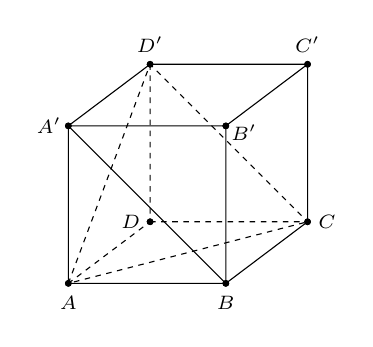
\begin{tikzpicture}[declare function={r=2;}]
				\path (0:0) coordinate (A) 
					(0:r) coordinate  (B)
					++(37:{0.65*r}) coordinate  (C)
					++(180:r)  coordinate (D)
				\foreach \x in  {A,B,C,D}{(\x)++(90:r) coordinate (\x')};
				\draw[dash pattern=on 2pt off  2 pt] (D')--(D)--(A)
					 (D)--(C)--(D')--(A)--(C);
				\draw  (A)--(B)--(C)
					(A)--(A') 
					 (B)--(B')
					 (C)--(C')
					(A')--(B')--(C')--(D')--cycle (A')--(B); 
				\foreach \x  in {A,B,C,D,A',B',C',D'}
				\draw[fill]  (\x) circle (1pt);
				 \foreach \t/\g in {A/-90,B/-90,C/0,D/180,A'/180,B'/-20,C'/90,D'/90}{
					\draw[fill]  (\t) circle (1pt) node[shift={(\g:7pt)},font=\scriptsize]{$ \t $};
				} 
			\end{tikzpicture}
		 }
	} 
\end{ex}

% từ: cau-hoi/lop12/2D1_Ung_dung_dao_ham_de_khao_sat_ham_so/2D1-1-1_Xet_tinh_don_dieu_cua_ham_so_cho_boi_cong_thu.tex
\begin{bt}%[2D1H1-1]%[ma:04229021]
% nguon: Archive/2024/0. [LVH] BG - 12 New - 4in1-20240625T224301Z-001/0. [LVH] BG - 12 New - 4in1/2. [LVH] TEX SGK 12 NEW-20240418T074833Z-001/2. [LVH] TEX SGK 12 NEW/[LVH] SGK-12-KNTT/data/C1/12-SGK-KNTT-1-3.tex #1100

	Đường thẳng $x=1$ có phải là tiệm cận đứng của đồ thị hàm số $y=\dfrac{x^2+2 x-3}{x-1}$ không?
	
	\loigiai{Ta có:\\
		$\begin{aligned} 
			&\lim _{x \rightarrow 1^{+}}f(x)=\lim _{x \rightarrow 1^{+}}\dfrac{x^2+2 x-3}{x-1}=\lim _{x \rightarrow 1^{+}}\dfrac{(x-1)(x+3)}{x-1}=\lim _{x \rightarrow 1^{+}}(x+3)=4;\\
			&  \lim _{x \rightarrow 1^{-}}f(x)=\lim _{x \rightarrow 1^{-}}\dfrac{x^2+2 x-3}{x-1}=\lim _{x \rightarrow 1^{-}}\dfrac{(x-1)(x+3)}{x-1}=\lim _{x \rightarrow 1^{-}}(x+3)=4.
		\end{aligned}$\\
		Suy ra đường thẳng $x=1$ không phải là tiệm cận đứng của đồ thị hàm số $y=\dfrac{x^2+2 x-3}{x-1}$.
	}
\end{bt}

% từ: cau-hoi/lop12/2D1_Ung_dung_dao_ham_de_khao_sat_ham_so/2D1-1-4_Ung_dung_tinh_don_dieu_de_chung_minh_bat_dang.tex
\begin{bt}%[2D1H1-4]%[ma:b64cbff5]
% nguon: Archive/2024/TaiLieuGiangDay/1.HamSo/1. K12 - 4in1 - Hamso/ThubaiGoc/Bai1-Dang4.tex #2645
%%[Mức độ 2]%[Dự án bài giảng new 4in1, Trần Quang Thạnh]
	Giải phương trình $3^x - 3^{x^2-2x} =x^2-3x$.
	\loigiai{
	Phương trình được biến đổi trở thành $3^x + x = 3^{x^2-2x}+x^2-2x$.\\
	Vì hàm số $y=f(t)=3^t$ đồng biến trên $\mathbb{R}$ nên từ phương trình trên ta được
	$$f(x)=f(x^2-2x) \Leftrightarrow x= x^2-2x \Leftrightarrow \hoac{&x=0\\ &x=3.}$$
	Vậy phương trình đã cho có tập nghiệm là $S=\{0;3\}$.
	}
\end{bt}

% từ: cau-hoi/lop12/2D1_Ung_dung_dao_ham_de_khao_sat_ham_so/2D1-1-4_Ung_dung_tinh_don_dieu_de_chung_minh_bat_dang.tex
\begin{bt}%[2D1C1-4]%[ma:c206efa8]
% nguon: Archive/2024/TaiLieuGiangDay/1.HamSo/1. K12 - 4in1 - Hamso/ThubaiGoc/Bai1-Dang4.tex #2647
%%[Mức độ 2]%[Dự án bài giảng new 4in1, Trần Quang Thạnh]
	Giải phương trình $\log_2 \dfrac{(x+1)^2}{2x} +x^2+1=0$.
	\loigiai{
		Điều kiện $x>0$.\\
		Ta thực hiện biến đổi như sau
		$$\log_2(x+1)^2 -\log_2 2x +(x+1)^2-2x=0 \Leftrightarrow \log_2(x+1)^2 +(x+1)^2 =\log_2 2x +2x.$$
		Vì hàm số $f(x)=\log_{2} t$ đồng biến trên khoảng $(0;+\infty)$ nên từ phương trình trên ta được
		$$f\left((x+1)^2\right)=f(2x) \Leftrightarrow (x+1)^2=2x \Leftrightarrow x^2+1 =0.$$
		Vậy phương trình đã cho vô nghiệm.
	}
\end{bt}

% từ: cau-hoi/lop12/2D1_Ung_dung_dao_ham_de_khao_sat_ham_so/2D1-1-4_Ung_dung_tinh_don_dieu_de_chung_minh_bat_dang.tex
\begin{bt}%[2D1H1-4]%[ma:9242e3cb]
% nguon: Archive/2024/TaiLieuGiangDay/1.HamSo/1. K12 - 4in1 - Hamso/ThubaiGoc/Bai1-Dang4.tex #2648
%%[Mức độ 2]%[Dự án bài giảng new 4in1, Trần Quang Thạnh]
	Giải phương trình $x+\log (x-3)=4$.
	\loigiai{
		Điều kiện xác định $x>3 $.\\
		Xét hàm số $ f(x)=x+\log (x-3) $ trên khoảng $ (3;+\infty ) $.\\
		Ta có cơ số $ 10>1 $ và hàm số $ y=x $ đồng biến nên $ f(x) $ đồng biến trên khoảng $ (3;+\infty) $.\\
		Mà $f(x)=f(4)=4\Leftrightarrow x=4 $ (thỏa mãn điều kiện xác định).\\
		Vậy $ x=4 $ là nghiệm duy nhất của phương trình.
	}
\end{bt}

% từ: cau-hoi/lop12/2D1_Ung_dung_dao_ham_de_khao_sat_ham_so/2D1-1-4_Ung_dung_tinh_don_dieu_de_chung_minh_bat_dang.tex
\begin{bt}%[2D1H1-4]%[ma:2a3a62f6]
% nguon: Archive/2024/TaiLieuGiangDay/1.HamSo/1. K12 - 4in1 - Hamso/ThubaiGoc/Bai1-Dang4.tex #2649
%%[Mức độ 2]%[Dự án bài giảng new 4in1, Trần Quang Thạnh]
	Giải phương trình $ \log_{3}(x+1)+\log_{2}x=2$.
	\loigiai{
		Điều kiện xác định $ x>0$.\\
		Xét hàm số $f(x)=\log_{3}(x+1)+\log_{2}x $ trên khoảng $\left(0;+\infty \right) $.\\
		Với $x>0$, ta có $f'(x)=\dfrac{1}{x\ln3}+\dfrac{1}{x\ln2}>0$, $\forall x>0$ nên hàm số $f(x)$ đồng biến trên $(0;+\infty)$.\\
		Mà $f(2)=2$ nên từ phương trình ta có $f(x)=f(2)\Leftrightarrow x=2 $ (thỏa mãn điều kiện xác định).\\
		Vậy $ x=2 $ là nghiệm của phương trình.
	}
\end{bt}

% từ: cau-hoi/lop12/2D1_Ung_dung_dao_ham_de_khao_sat_ham_so/2D1-1-4_Ung_dung_tinh_don_dieu_de_chung_minh_bat_dang.tex
\begin{bt}%[2D1H1-4]%[ma:4d4eef8b]
% nguon: Archive/2024/TaiLieuGiangDay/1.HamSo/1. K12 - 4in1 - Hamso/Thubai/Bai1-Dang4_converted_converted.tex #2963
%%[Mức độ 2]%[Dự án bài giảng new 4in1, Trần Quang Thạnh]
Giải phương trình $5^x-5^{2x+1}=x+1$.
\loigiai{
Phương trình đã cho tương đương với $5^x + x =5^{2x+1}+2x+1$.\\
Vì hàm số $y=f(t)=5^t+t$ có $y'=5^t\ln5 +1 > 0$, với mọi $t\in \mathbb{R}$ nên hàm số $y=f(t)$ đồng biến trên $\mathbb{R}$, do đó, từ phương trình đã cho ta được $$f(x)=f(2x+1) \Leftrightarrow x=2x+1 \Leftrightarrow x=-1.$$
Vậy phương trình đã cho có nghiệm duy nhất $x=-1$.
}
\end{bt}

% từ: cau-hoi/lop12/2D1_Ung_dung_dao_ham_de_khao_sat_ham_so/2D1-1-4_Ung_dung_tinh_don_dieu_de_chung_minh_bat_dang.tex
\begin{bt}%[2D1H1-4]%[ma:c18f3620]
% nguon: Archive/2024/TaiLieuGiangDay/1.HamSo/1. K12 - 4in1 - Hamso/Thubai/Bai1-Dang4_converted_converted.tex #2964
%%[Mức độ 2]%[Dự án bài giảng new 4in1, Trần Quang Thạnh]
Giải bất phương trình $\log x > \log (2x-1) + x-1$.
\loigiai{
Điều kiện $x > \dfrac{1}{2}$.\\
Bất phương trình đã cho tương đương với
$\log x + x > \log(2x-1) +2x-1$.\\
Vì hàm số $y=f(t)=\log t + t$ có $y'=\dfrac{1}{t\ln10}+1 > 0$, với mọi $t > 0$ nên hàm số $y=f(t)$ đồng biến trên $(0;+\infty)$.\\
Do đó, từ bất phương trình đã cho ta được
$$f(x) > f(2x-1) \Leftrightarrow x > 2x-1 \Leftrightarrow x < 1.$$
Kết hợp điều kiện, ta có tập nghiệm bất phương trình là $S=\left(\dfrac{1}{2};1\right)$.
}
\end{bt}

% từ: cau-hoi/lop12/2D1_Ung_dung_dao_ham_de_khao_sat_ham_so/2D1-3-1_GTLN_GTNN_tren_doan.tex
\begin{ex}%[2D1N3-1]%[ma:5bd97acc]
	Đồ  thị hàm số $y=\dfrac{x-2}{x^{2}-4}$ có mấy đường tiệm cận?
	\choice 
		{$3$} 
		 {$1$}
		 {\True$2$}
		 {$0$}
	\loigiai{Ta có  $y = \dfrac{x-2}{x^{2}-4} = \dfrac{x-2}{(x-2)(x+2)}= \dfrac{1}{x+2}$.\\
		Do $\heva{&\displaystyle\lim_{x\to +\infty  }\dfrac{1}{x+2}=0\\&
		\displaystyle\lim_{x\to -\infty }\dfrac{1}{x+2}=0}$. Suy  ra đường thẳng $y=0$ là tiệm cận ngang của hàm số.\\
		Đồ  thị hàm số có tiệm cận ngang thì không có tiệm cận xiên.\\
		Do $\heva{&\displaystyle\lim_{x\to -2^-  }\dfrac{1}{x+2}= - \infty \\&
		\displaystyle\lim_{x\to -2^+ }\dfrac{1}{x+2}= + \infty}$. Suy  ra đường thẳng $x=-2$ là tiệm cận đứng của hàm số.\\
		Vậy hàm số có hai đường tiệm cận. 
	} 
\end{ex}

% từ: cau-hoi/lop12/2D1_Ung_dung_dao_ham_de_khao_sat_ham_so/2D1-3-1_GTLN_GTNN_tren_doan.tex
\begin{ex}%[2D1N3-1]%[ma:f5843a1d]
	Đường thẳng $ y = m $  được gọi là một đường tiệm cận ngang (hay tiệm cận ngang) của đồ thị hàm số $y = f (x)$ nếu
	 \choice
		{\True $\lim\limits_{x \to +\infty} f(x) = m$ hoặc $\lim\limits_{x  \to -\infty }f(x) = m$}
		{$\lim\limits_{x  \to \infty} f(x) = -m $ hoặc $\lim\limits_{x \to \infty }f(x) = -m $}
		{$\lim\limits_{x \to m} f(x)= +\infty$ hoặc $\lim\limits_{x \to  m }f(x) = -\infty $}
		{$\lim\limits_{x \to -m}  f(x) = +\infty$ hoặc $\lim\limits_{x \to -m} f(x) = -\infty $}
	\loigiai{Đường thẳng $y = m$ được gọi là một đường tiệm cận ngang (hay tiệm cận ngang) của đồ thị hàm số $y =  f (x) $ nếu $\lim\limits_{x\to +\infty} f(x) = m$ hoặc $\lim\limits_{x\to -\infty} f(x) = m$.
	 }
\end{ex}

% từ: cau-hoi/lop12/2D1_Ung_dung_dao_ham_de_khao_sat_ham_so/2D1-3-1_GTLN_GTNN_tren_doan.tex
\begin{ex}%[2D1N3-1]%[ma:be38ac7f]
	Đường thẳng $x = a$ được gọi là  một đường tiệm cận đứng (hay tiệm cận đứng) của đồ thị hàm số $ y = f (x)$ nếu điều kiện sau thoả mãn
	\choice 
		 {$\lim\limits_{x\to +\infty }f(x)=a$}
		 {\True $\lim\limits_{x\to a^-}f(x)=+\infty $}
		{$\lim\limits_{x\to -\infty }f(x)=a$} 
		{$\lim\limits_{x\to  a^-}f(x)=a $}
	\loigiai{Đường thẳng $x = a$ được gọi là một đường tiệm cận đứng của đồ thị hàm số $y = f (x)$ nếu ít nhất một trong các điều kiện sau thoả mãn $$\lim\limits_{x\to a^+} f(x) = +\infty, \lim\limits_{x\to a^+} f(x) = -\infty, \lim\limits_{x \to a^-}f(x) = -\infty , \lim\limits_{x\to a^-} f(x)  = +\infty .$$
	 }
\end{ex}

% từ: cau-hoi/lop12/2D1_Ung_dung_dao_ham_de_khao_sat_ham_so/2D1-3-1_GTLN_GTNN_tren_doan.tex
\begin{ex}%[2D1N3-1]%[ma:ecdd7b5a]
	Cho hàm số  $y=f(x)$ thoả mãn $\lim\limits_{x \to - \infty } [f(x)-5x+7]=0$. Đường tiệm cận xiên của đồ thị hàm số $y=f(x)$ là
	 \choice
		 {\True $y=5x-7$}
		 {$y=5x+7$}
		 {$y=-5x-7$}
		 {$y=5x+7$}
	\loigiai{ 
		Vì $\lim\limits_{x \to - \infty} [f(x)-5x+7]=0\Leftrightarrow \lim\limits_{x \to -\infty} [f(x)-(5x-7)]=0$ nên  đồ thị hàm số có tiệm cận xiên là $y=5x-7$.
	} 
\end{ex}

% từ: cau-hoi/lop12/2D1_Ung_dung_dao_ham_de_khao_sat_ham_so/2D1-3-1_GTLN_GTNN_tren_doan.tex
\begin{ex}%[2D1N3-1]%[ma:ede13f5a]
	Đường thẳng $y = ax + b, a \neq 0$, được  gọi là đường tiệm cận xiên (hay tiệm cận xiên) của đồ thị hàm số $y = f(x)$ nếu
	\choice 
		{\True $\lim\limits_{x\to -\infty }(f(x)-ax-b)=0$ hoặc $\lim\limits_{x\to +\infty }(f(x)-ax-b)=0$} 
		 {$\lim\limits_{x\to -\infty }(f(x)-ax+b)=0$ hoặc $\lim\limits_{x\to +\infty }(f(x)-ax+b)=0$}
		{$\lim\limits_{x\to 0  }[f(x)-(ax+b)]=+\infty $ hoặc $\lim\limits_{x\to 0 }[f(x)-(ax+b)]=-\infty $}
		{$\lim\limits_{x\to -\infty }(f(x)-ax+b)=a$  hoặc $\lim\limits_{x\to +\infty }(f(x)-ax+b)=a$}
	\loigiai{Đường thẳng $y = ax + b, a \neq 0$, được gọi là đường tiệm cận xiên  (hay tiệm cận xiên) của đồ thị hàm số $y = f(x)$ nếu\\ $\lim\limits_{x\to -\infty }[f(x)-(ax+b)] = \lim\limits_{x\to -\infty} (f(x)-ax-b) = 0$ hoặc\\ $\lim\limits_{x\to +\infty }[f(x)-(ax+b)] = \lim\limits_{x \to +\infty }(f(x)-ax-b) = 0$.
	 }
\end{ex}

% từ: cau-hoi/lop12/2D1_Ung_dung_dao_ham_de_khao_sat_ham_so/2D1-3-1_GTLN_GTNN_tren_doan.tex
\begin{ex}%[2D1N3-1]%[ma:0456acba]
	Cho hàm số phù hợp với bảng biến thiên sau 
	\begin{center}
		
\begin{tikzpicture}
			\tkzTabInit[nocadre,lgt=1.5,espcl=2.5] 
				{$x$ /1,$y'$ /1,$y$  /2}
				 {$-\infty$,$2$,$+\infty$}
			\tkzTabLine{,+,0,-} 
			\tkzTabVar{-/$-1$,+/ $1$ /,-/$1$} 
		\end{tikzpicture}
	\end{center}
	Phát biểu nào sau đây là  đúng?
	\choice 
		{\True Đồ thị hàm số có hai đường tiệm  cận ngang là $y=-1$, $y=1$}
		{Đồ thị hàm  số có hai đường tiệm cận ngang là $x=-1$, $x=1$}
		{Đồ thị hàm  số không có đường tiệm cận ngang}
		{Đồ thị hàm  số có đường tiệm cận đứng}
	\loigiai{ 
		Vì $\lim\limits_{x \to - \infty } f(x)=-1$; $\lim\limits_{x \to +\infty} f(x)=1$ nên đồ thị hàm  số có haitiệm cận ngang là $y=-1$ và $y=1$.
	 }
\end{ex}

% từ: cau-hoi/lop12/2D1_Ung_dung_dao_ham_de_khao_sat_ham_so/2D1-3-1_GTLN_GTNN_tren_doan.tex
\begin{ex}%[2D1H3-1]%[ma:d32100d4]
	Cho hàm số $f(x)$ xác định và liên tục trên $\mathbb{R}\setminus \{-1\}$  có bảng biến thiên như sau
	\begin{center}
		
\begin{tikzpicture}
			 \tkzTabInit[lgt=1.5,espcl=4,deltacl=.5]
				 {$x$/0.7,$f’(x)$/0.7,$f (x)$/2}
				 {$-\infty$,$-1$,$+\infty$}
			\tkzTabLine{,-,d,-,} 
			 \tkzTabVar{+/$5$,-D+/ $-\infty$/$+\infty$,-/$2$}
		\end{tikzpicture}
	\end{center}
	Khẳng định nào sau đây đúng? 
	 \choice
		{\True Đồ thị hàm số $f(x)$ có hai tiệm cận ngang  là các đường thẳng $y=2$, $y=5$ và có một tiệm cận đứng là đường thẳng $x=-1$}
		{Đồ  thị hàm số có bốn đường tiệm cận}
		{Đồ thị hàm số có  hai đường tiệm cận}
		{Đồ thị hàm số có một  đường tiệm cận}
	\loigiai{ 
		Dựa vào bảng biên thiên ta thấy hàm số $f(x)$ có 3 đường tiệm cận đó là hai tiệm cận ngang $y=2$, $y=5$  và có một tiệm cận đứng là đường thẳng $x=-1$.
	} 
\end{ex}

% từ: cau-hoi/lop12/2D1_Ung_dung_dao_ham_de_khao_sat_ham_so/2D1-3-1_GTLN_GTNN_tren_doan.tex
\begin{ex}%[2D1H3-1]%[ma:799aaf1b]
	Tiệm cận xiên của đồ thị hàm số $f(x)  = \dfrac{x^2+x-1}{x}$ là đường thẳng
	\choice 
		 {$y=x-1$}
		 {$y=x-2$}
		{$y=x-3$} 
		 {\True$y=x+1$}
	\loigiai{Gọi đường thẳng $y=ax+b, a\neq 0$ là đường tiệm cận xiên của hàm  số\\
		Ta có $a=\displaystyle\lim_{x\to +\infty  }\dfrac{\dfrac{x^2+x-1}{x}}{x}=1$.;
		$b=\displaystyle\lim_{x\to  +\infty }\left[\dfrac{x^2+x-1}{x}-x \right]=1$.\\
		Vậy đường tiệm cận  xiên cần tìm của đồ thị hàm số $f(x)$ có phương trình $y=x+1$.
	 }
\end{ex}

% từ: cau-hoi/lop12/2D1_Ung_dung_dao_ham_de_khao_sat_ham_so/2D1-3-1_GTLN_GTNN_tren_doan.tex
\begin{ex}%[2D1V3-1]%[ma:81ae365f]
	 Đồ thị hàm số $y = \dfrac{2x}{\sqrt{x^2-1}}$ có số đường tiệm cận là
	 \choice
		{$2$} 
		 {$1$}
		{$3$} 
		{\True$4$} 
	\loigiai{Ta có $\lim\limits_{x\to +\infty }\dfrac{2x}{\sqrt{x^2-1}} = \lim\limits_{x\to +\infty }\dfrac{2x}{|x|\sqrt{1-\dfrac{1}x^2}} =  \lim\limits_{x\to +\infty }\dfrac{2x}{x\sqrt{1-\dfrac{1}x^2}} = \lim\limits_{x\to +\infty }\dfrac{2}{\sqrt{1-\dfrac{1}x^2}}=2$.\\
		$\lim\limits_{x\to -\infty }\dfrac{2x}{\sqrt{x^2-1}}=\lim\limits_{x\to -\infty} \dfrac{2x}{|x|\sqrt{1-\dfrac{1}x^2}} = \lim\limits_{x\to -\infty} \dfrac{2x}{-x\sqrt{1-\dfrac{1}x^2}} =  \lim\limits_{x\to -\infty} \dfrac{-2}{\sqrt{1-\dfrac{1}x^2}}=-2$.\\
		Suy ra $y=-2$ và $y=2$ là phương trình  hai đường tiệm cận ngang của đồ thị hàm số đã cho.\\
		Mặt khác $\lim\limits_{x\to 1^-} y =  \lim\limits_{x\to (-1)^-} \dfrac{2x}{\sqrt{x^2-1}} = -\infty$; $\lim\limits_{x\to 1^+}y = \lim\limits_{x\to 1^+} \dfrac{2x}{\sqrt{x^2-1}} = +\infty$.\\
		Nên đồ thị hàm số có hai tiệm  cận đứng là đường thẳng $x=-1$ và đường thẳng $x=1$.\\
		 Vậy đồ thị hàm số có $4$ tiệm cận.
	 }
\end{ex}

% từ: cau-hoi/lop12/2D1_Ung_dung_dao_ham_de_khao_sat_ham_so/2D1-3-1_GTLN_GTNN_tren_doan.tex
\begin{bt}%[2D1H3-1]%[ma:0ac3ce0c]
	Đồ thị hàm số $y = \dfrac{x-3}{x^2+x-2}$ có  bao nhiêu đường tiệm cận đứng?
	 \shortans{2}
	\loigiai{Ta có $\heva{&\lim\limits_{x\to 1^+}y=\dfrac{x-3}{x^2+x-2}= -\infty\\&\lim\limits_{x\to 1^-}y=\dfrac{x-3}{x^2+x-2}= +\infty} \Rightarrow$ đường  thẳng $x=1$ là tiệm cận đứng của đồ thị hàm số.\\
		Mặt khác $\heva{&\lim\limits_{x\to 2^+} y = \dfrac{x-3}{x^2+x-2} = +\infty\\& 
		\lim\limits_{x\to 2^-} y = \dfrac{x-3}{x^2+x-2} =  -\infty} \Rightarrow$
		đường thẳng $x=-2$ là tiệm cận đứng của  đồ thị hàm số.\\
		Vậy đồ thị hàm số có hai đường tiệm cận đứng. 
	} 
\end{bt}

% từ: cau-hoi/lop12/2D1_Ung_dung_dao_ham_de_khao_sat_ham_so/2D1-3-1_GTLN_GTNN_tren_doan.tex
\begin{bt}%[2D1C3-1]%[ma:df981945]
	Số giá trị nguyên của tham số $m$ để hàm số $y = \dfrac{1 + \sqrt{x + 1}}{x^2 - (1-m)x + 2m}$ có $3$ đường tiệm cận  (bao gồm tiệm cận đứng và tiệm cận ngang) là
	\shortans{2} 
	\loigiai{ 
		Điều kiện xác định $\heva{&x  \geq -1\\&x^2 - (1-m)x + 2m \neq 0}.$\\
		Ta  có $y = \dfrac{1 + \sqrt{x+1}}{x^2 - (1-m)x + 2m.}$\\
		 Đồ thị hàm số $y=\dfrac{1+\sqrt{x+1}}{x^2-(1-m)x+2m}$ với $x \geq-1$ có tiệm cận ngang là đường thẳng $y=0$.\\
		Do đó để đồ thị  hàm số có $3$ đường tiệm cận thì đồ thị hàm số phải có $2$ tiệm cận đứng.\\
		Khi đó phương trình $x^2-(1-m)x+2m=0$ có $2$ nghiệm phân biệt lớn  hơn $-1$\\
		$\Leftrightarrow \heva{&\Delta > 0\\&(x_1 + 1)(x_2 + 1) > 0\\&x_1 + 1 + x_2 + 1 >  0} \Leftrightarrow \heva{&(1-m)^2-8m>0\\&x_1x_2 + (x_1 + x_2) + 1 > 0\\&x_1 + x_2 + 2 > 0} \Leftrightarrow \heva{&1 - 2m + m^2 - 8m > 0\\&2m + 1 - m + 1 > 0\\&1 - m + 2 > 0}$\\
		$\Leftrightarrow \heva{&1 - 2m + m^2 - 8m > 0\\&m + 2 > 0\\&m < 3} \Leftrightarrow \heva{&m^2 - 10m + 1 > 0\\&m > -2\\&m < 3} \Leftrightarrow \heva{&\hoac{&m  > 5 + 2\sqrt{6}\\&m < 5 - 2\sqrt{6}}\\&-2 < m < 3}$ \\$ \Leftrightarrow -2 < m < 5 - 2\sqrt{6}$.\\
		Vậy $m\in\{-1;0\}$. Suy ra có $2$ giá trị $m$ thỏa  mãn.
	 }
\end{bt}

% từ: cau-hoi/lop12/2D3_Cac_so_dac_trung_ghep_nhom/2D3-1-1_Cong_thuc_ly_thuyet.tex
\begin{bt}%[2D3H1-1]%[ma:87c6da6f]
	Biết hàm  số $F(x)$ là một nguyên hàm của hàm số $f(x)=2^x+3 x^2$ và $F(1)=\dfrac{2}{\ln 2}$. Giá trị của $F(2)$ (làm tròn đến hàng phần mười) bằng
	 \shortans{12,8}
	\loigiai{ 
		Ta  có
		\[ 
		\displaystyle\int f(x)\mathrm{\,d}x 
		=\displaystyle\int\left(2^x+3  x^2\right)\mathrm{\,d}x
		=\dfrac{2^x}{\ln  2}+x^3+C.
		\] 
		Suy ra  $F(x)=\dfrac{2^x}{\ln 2}+x^3+C$.
		\\ 
		Ta có $F(1)=\dfrac{2}{\ln 2}+1+C=\dfrac{2}{\ln 2} \Rightarrow  C=-1$.
		 \\
		 Do đó $F(2)=\dfrac{2^2}{\ln 2}+2^3-1 \approx 12{,}8$.
	} 
\end{bt}

% từ: cau-hoi/lop12/2D4_Nguyen_ham_tich_phan/2D4-2-2_Tich_phan_co_ban_da_thuc_phan_thuc.tex
\begin{ex}%[2D4N2-2]%[ma:b997c0d6]
	Họ các nguyên hàm của hàm số $f(x)=3x^2-4x$  là
	\choice 
		{$F(x)=6x-4+C$} 
		{$F(x)=x^3+2x^2+C$} 
		 {\True$F(x)=x^3-2x^2+C$}
		 {$F(x)=x^3-4+C$}
	\loigiai{Ta có $f(x)=\displaystyle \int f(x)\mathrm{\,d}x=\displaystyle \int \left(3x^2-4x\right)\mathrm{\,d}x=x^3-2x^2+C$.} 
\end{ex}

% từ: cau-hoi/lop12/2D4_Nguyen_ham_tich_phan/2D4-2-6_Toan_thuc_te_ap_dung_nguyen_ham.tex
\begin{ex}%[2D4V2-6]%[ma:cb084147]
	\immini{Cho hàm số $y=f(x)$ có đồ thị $y=f'(x)$ cắt trục $Ox$ tại ba điểm có hoành độ $a<b<c$  như hình vẽ. Mệnh đề nào sau đây là đúng?
	\choice 
		{\True  $f(c)>f(a)>f(b)$}
		{$f(c)>f(b)>f(a)$} 
		{$f(a)>f(b)>f(c)$} 
		{$f(b)>f(a)>f(c)$} 
		}{ 
		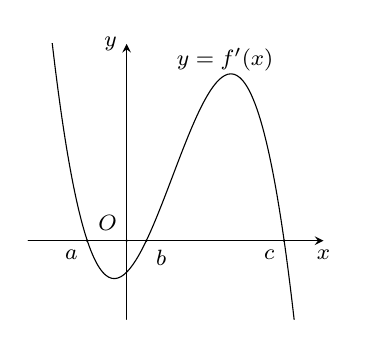
\begin{tikzpicture}[scale=0.5,line cap=round,line join=round,font=\footnotesize,>=stealth]
				\draw[->] (-2.5,0) -- (5,0) node[below]{$x$}; 
				\draw[->] (0,-2)  -- (0,5) node[left] {$y$};
				 \fill (0,0) circle (1pt) node[above left] {$O$}
					(-1,0) circle  (1pt) node[below left] {$a$}
					(0.5,0) circle (1pt) node[below  right] {$b$}
					(4,0)  circle (1pt) node[below left] {$c$};
				 \clip (-2.5,-2) rectangle (5,5);
				 \draw[smooth,samples=100,domain=-2.5:5] plot (\x,{0.4*((\x)+1)*(4-(\x))*((\x)-0.5)});
				\draw (2.5,4.6)  node{$y=f'(x)$};
			\end{tikzpicture}
		 }
	 \loigiai{
		Dựa  vào đồ thị hàm số $y=f'(x)$, ta có
		\allowdisplaybreaks 
		\begin{eqnarray*}
			\displaystyle \int_a^b f'(x) \mathrm{\,d}x < 0 &\Leftrightarrow& f(x) \Big|_a^b <0\\ 
			&\Leftrightarrow&  f(b)-f(a)<0\\
			&\Leftrightarrow& f(a)>f(b).  \quad (1)\\
			\displaystyle \int_b^c f'(x) \mathrm{\,d}x > 0 &\Leftrightarrow& f(x)  \Big|_b^c >0\\
			&\Leftrightarrow& f(c)-f(b)>0\\ 
			&\Leftrightarrow& f(c)>f(b).  \quad (2)\\
			 - \displaystyle \int_a^b f'(x) \mathrm{\,d}x < \displaystyle \int_b^c f'(x) \mathrm{\,d}x &\Leftrightarrow& -f(x) \Big|_a^b < f(x) \Big|_b^c\\
			 &\Leftrightarrow& f(a)-f(b) < f(c)-f(b)\\
			&\Leftrightarrow& f(a) < f(c). \quad  (3)
		\end{eqnarray*}
		Từ $(1)$, $(2)$ và $(3)$ suy ra $f(c)>f(a)>f(b)$. 
	 }
\end{ex}

% từ: cau-hoi/lop12/2H5_Phuong_trinh_mat_phang_duong_thang_mat_c/2H5-2-4_Vi_tri_tuong_doi_giua_hai_duong_thang.tex
\begin{ex}%[2H5H2-4]%[ma:74debd10]
	Cho hình chóp $S.ABCD$ có đáy $ABCD$ là tam giác vuông với $AB = AC = 2$. Cạnh bên $SA$ vuông góc với đáy và $SA = 3$. Gọi  $M$ là trung điểm của $SC$. Tính khoảng cách giữa $AM$ và $BC$.
	 \choice
		{$\dfrac{\sqrt{3}}{2}$} 
		 {$\dfrac{2\sqrt{3}}{3}$}
		{\True  $\dfrac{3\sqrt{22}}{11}$}
		 {$\dfrac{\sqrt{22}}{6}$}
	\loigiai{ 
		Đặt hệ trục tọa độ sao  cho $
		A(0;0;0)$, $ B(2;0;0)$,  $ C(0;2;0)$, $ S(0;0;3)$.\\
		Điểm $M \left(0;1;\dfrac{3}{2}\right)$,  ta có
		$ 
		 \overrightarrow{AM} = \left(0;1;\dfrac{3}{2}\right)$, $ \overrightarrow{BC} = (-2;2;0)$. \\
		Gọi 
		$ \overrightarrow{n} = \left[\overrightarrow{AM}, \overrightarrow{BC}\right] = (-3;  -3; 2)$.\\
		Mặt phẳng $(P)$ qua điểm $B(2;0;0)$ và nhận $\overrightarrow{n}$ làm véc-tơ pháp tuyến có  phương trình
		$$ 
		-3(x - 2) - 3y + 2z = 0 \Rightarrow -3x  - 3y + 2z + 6 = 0.
		 $$
		 Ta có
		 $$
		\mathrm{d}(AM, BC) = \mathrm{d}(A, (P)) = \dfrac{|-3\cdot 0 -3\cdot 0 + 2\cdot 0 + 6|}{\sqrt{(-3)^2 + (-3)^2 + 2^2}} = \dfrac{6}{\sqrt{22}} =  \dfrac{3\sqrt{22}}{11}.
		 $$
	} 
\end{ex}

% từ: cau-hoi/lop12/2H5_Phuong_trinh_mat_phang_duong_thang_mat_c/2H5-2-7_Goc_giua_hai_duong_thang_duong_thang_va_mat_p.tex
\begin{ex}%[2H5H2-7]%[ma:25f9ee36]
	Cho lăng trụ đứng $ABC.A'B'C'$ có đáy là tam giác $ABC$ vuông cân tại $A$, cạnh $BC = a\sqrt{6}$. Góc giữa mặt phẳng $(ABC')$  và mặt phẳng $(BCC'B')$ bằng $60^\circ$. Tính thể tích $V$ của khối lăng trụ $ABC.A'B'C'$.
	\loigiai{ 
		Gọi chiều cao của hình  lăng trụ là $h$.\\
		Đặt hệ trục tọa độ $Oxyz$ như hình vẽ.\\ 
		Khi đó  tọa độ các điểm
		$A(0;0;0)$, $  B\left(a\sqrt{3}; 0; 0\right)$, $C\left(0; a\sqrt{3}; 0\right)$, $ B'\left(a\sqrt{3}; 0; h\right)$.\\
		 $
		M\left(\dfrac{a\sqrt{3}}{2}; \dfrac{a\sqrt{3}}{2}; 0\right) \text{ là  trung điểm của } BC
		$. 
		\begin{center}
			\tdplotsetmaincoords{70}{110} 
			\begin{tikzpicture}[tdplot_main_coords,scale=2]
					 \coordinate (A) at (0,0,0);
					\coordinate  (B) at (1.5,0,0);
					\coordinate (C)  at (0,1.5,0);
					\coordinate  (M) at (0.75,0.75,0);
					 \coordinate (A') at (0,0,2);
					 \coordinate (B') at (1.5,0,2);
					\coordinate (C')  at (0,1.5,2);
					\draw[->] (1.5,0,0) -- (2.5,0,0) node[below]  {$x$};
					 \draw[->] (0,1.5,0) -- (0,2.5,0) node[above] {$y$};
					\draw[->] (0,0,2) -- (0,0,2.5) node[above]  {$z$};
					 \draw[dashed] (B) -- (A) -- (C);
					\draw[dashed] (A') -- (A) --  (M);
					\draw  (B) -- (C);
					\draw (A') -- (B') -- (C') -- cycle; 
					\draw[dashed] (A) --  (A') node[above left] {$A'$};
					\draw (B) -- (B') node[above]  {$B'$};
					\draw (C) --  (C') node[above right] {$C'$};
					\draw (B') --  (C);
					\draw (C')  -- (B);
					\fill  (A) circle (1pt) node[above right] {$A$};
					\fill (B) circle (1pt) node[below] {$B$}; 
					\fill (C) circle (1pt) node[below right] {$C$}; 
					\fill (M) circle  (1pt) node[below right] {$M$};
					 \fill (A') circle (1pt);
					\fill (B') circle  (1pt);
					\fill (C')  circle (1pt);
				\end{tikzpicture}
		\end{center}
		Vì $AM \perp (BCC'B')$ và $\overrightarrow{AM} =  \left(\dfrac{a\sqrt{3}}{2}; \dfrac{a\sqrt{3}}{2}; 0\right)$, nên $\overrightarrow{n} = (1;1;0)$ là véc-tơ pháp tuyến của mặt phẳng $(BCC'B')$.\\
		Ta  có
		$$ 
		\left[\overrightarrow{AC}, \overrightarrow{AB'}\right] =  \left[(0;a\sqrt{3};0), \left(a\sqrt{3};0;h\right)\right] = \left(ah\sqrt{3};0; -3a^2\right).
		 $$
		Suy ra $\overrightarrow{n}_1 = \left(h; 0; -\sqrt{3}a\right)$ là  véc-tơ pháp tuyến của mặt phẳng $(ABC')$.\\
		Theo giả thiết, góc giữa  hai mặt phẳng là $60^\circ$, ta có
		$$ 
		\cos 60^\circ = \left|\cos(\overrightarrow{n}, \overrightarrow{n}_1)\right| = \left|\dfrac{\overrightarrow{n} \cdot  \overrightarrow{n}_1}{\left|\overrightarrow{n}\right|\cdot \left|\overrightarrow{n}_1\right|}\right| = \dfrac{1}{2}
		\Rightarrow \dfrac{h}{\sqrt{2} \cdot \sqrt{h^2 + 3a^2}} = \dfrac{1}{2} \Rightarrow h =  \sqrt{3}a.
		$$ 
		Vậy  thể tích khối lăng trụ
		 $$
		V = S_{\text{đáy}} \cdot h = \dfrac{1}{2} \cdot AB \cdot AC \cdot h  = \dfrac{1}{2} \cdot a\sqrt{3} \cdot a\sqrt{3} \cdot \sqrt{3}a = \dfrac{3a^3\sqrt{3}}{2}.
		$$ 
	 }
\end{ex}

% từ: cau-hoi/lop12/2H5_Phuong_trinh_mat_phang_duong_thang_mat_c/2H5-2-7_Goc_giua_hai_duong_thang_duong_thang_va_mat_p.tex
\begin{bt}%[2H5H2-7]%[ma:45970cd0]
	Cho lăng trụ đứng $ABC.A'B'C'$ có đáy là tam giác $ABC$ vuông cân tại $A$, cạnh $BC = a\sqrt{6}$. Góc giữa mặt phẳng $(ABC')$ và mặt phẳng $(BCC'B')$ bằng $60^\circ$. Tính thể tích  $V$ của khối lăng trụ $ABC.A'B'C'$.
	\loigiai{ 
		Gọi chiều cao của hình lăng trụ  là $h$.\\
		 Đặt hệ trục tọa độ $Oxyz$ như hình vẽ.\\
		Khi đó  tọa độ các điểm
		$A(0;0;0)$, $  B\left(a\sqrt{3}; 0; 0\right)$, $C\left(0; a\sqrt{3}; 0\right)$, $ B'\left(a\sqrt{3}; 0; h\right)$.\\
		 $
		M\left(\dfrac{a\sqrt{3}}{2}; \dfrac{a\sqrt{3}}{2}; 0\right) \text{ là trung điểm của } BC 
		$. 
		\begin{center}
			\tdplotsetmaincoords{70}{110} 
			\begin{tikzpicture}[tdplot_main_coords,scale=2]
					\coordinate  (A) at (0,0,0);
					\coordinate (B) at (1.5,0,0); 
					\coordinate (C) at (0,1.5,0); 
					\coordinate (M)  at (0.75,0.75,0);
					\coordinate (A') at  (0,0,2);
					\coordinate (B') at (1.5,0,2); 
					\coordinate  (C') at (0,1.5,2);
					\draw[->] (1.5,0,0) -- (2.5,0,0) node[below] {$x$}; 
					 \draw[->] (0,1.5,0) -- (0,2.5,0) node[above] {$y$};
					\draw[->] (0,0,2) -- (0,0,2.5)  node[above] {$z$};
					\draw[dashed]  (B) -- (A) -- (C);
					\draw[dashed] (A') --  (A) -- (M);
					\draw (B) -- (C); 
					\draw  (A') -- (B') -- (C') -- cycle;
					\draw[dashed] (A) --  (A') node[above left] {$A'$};
					\draw (B)  -- (B') node[above] {$B'$};
					\draw (C)  -- (C') node[above right] {$C'$};
					\draw (B') --  (C);
					\draw  (C') -- (B);
					\fill (A) circle (1pt) node[above  right] {$A$};
					\fill (B) circle (1pt) node[below]  {$B$};
					\fill (C) circle (1pt) node[below  right] {$C$};
					\fill (M)  circle (1pt) node[below right] {$M$};
					\fill (A')  circle (1pt);
					\fill (B') circle (1pt); 
					 \fill (C') circle (1pt);
				\end{tikzpicture}
		\end{center}
		Vì $AM \perp (BCC'B')$ và $\overrightarrow{AM} = \left(\dfrac{a\sqrt{3}}{2}; \dfrac{a\sqrt{3}}{2}; 0\right)$, nên $\overrightarrow{n}  = (1;1;0)$ là véc-tơ pháp tuyến của mặt phẳng $(BCC'B')$.\\
		Ta  có
		$$ 
		\left[\overrightarrow{AC}, \overrightarrow{AB'}\right] = \left[(0;a\sqrt{3};0), \left(a\sqrt{3};0;h\right)\right]  = \left(ah\sqrt{3};0; -3a^2\right).
		$$ 
		Suy ra $\overrightarrow{n}_1 = \left(h; 0; -\sqrt{3}a\right)$ là véc-tơ pháp tuyến của mặt phẳng  $(ABC')$.\\
		Theo giả thiết, góc giữa  hai mặt phẳng là $60^\circ$, ta có
		$$ 
		\cos 60^\circ = \left|\cos(\overrightarrow{n}, \overrightarrow{n}_1)\right| = \left|\dfrac{\overrightarrow{n}  \cdot \overrightarrow{n}_1}{\left|\overrightarrow{n}\right|\cdot \left|\overrightarrow{n}_1\right|}\right| = \dfrac{1}{2}
		\Rightarrow \dfrac{h}{\sqrt{2} \cdot \sqrt{h^2 + 3a^2}} = \dfrac{1}{2}  \Rightarrow h = \sqrt{3}a.
		 $$
		Vậy thể tích khối lăng  trụ
		 $$
		V = S_{\text{ đáy}} \cdot h = \dfrac{1}{2} \cdot AB \cdot AC \cdot h = \dfrac{1}{2} \cdot a\sqrt{3} \cdot a\sqrt{3} \cdot \sqrt{3}a = \dfrac{3a^3\sqrt{3}}{2}. 
		 $$
	 }
\end{bt}

% từ: cau-hoi/lop8/8D1_Chuong_I_Da_thuc/8D1-3-1_Cong_tru_hai_da_thuc.tex
\begin{bt}%[8D1H3-1]%[ma:c10694b2]
	Rút gọn các biểu thức sau:
a) $P = x(2x - y) + y(x - 2y)$;
b) $Q = 3x(x - 2y) - (x - y)(3x - 2y)$.
	\loigiai{
		a) $P = 2x^2 - xy + xy - 2y^2 = 2x^2 - 2y^2$. \\
b) $Q = (3x^2 - 6xy) - (3x^2 - 2xy - 3xy + 2y^2) = 3x^2 - 6xy - 3x^2 + 5xy - 2y^2 = -xy - 2y^2$.
	}
\end{bt}

% từ: cau-hoi/lop8/8D2_Chuong_II_Hang_dang_thuc_dang_nho_va_ung/8D2-6-4_Chung_minh_dang_thuc_tim_gia_tri_nho_nhat_lon.tex
\begin{bt}%[8D2N6-4]%[ma:c7b7a3d7]
	Chứng minh rằng giá trị của biểu thức $K = (x + 5)^2 - x(x + 10)$ không phụ thuộc vào giá trị của biến $x$.
	\loigiai{
		Ta có $K = (x + 5)^2 - x(x + 10) = (x^2 + 10x + 25) - (x^2 + 10x) = x^2 + 10x + 25 - x^2 - 10x = 25$. \\
Vì $K = 25$ là một hằng số nên giá trị của $K$ không phụ thuộc vào giá trị của biến $x$.
	}
\end{bt}
